\documentclass[conference]{IEEEtran}
\IEEEoverridecommandlockouts
\usepackage{cite}
\usepackage{amsmath,amssymb,amsfonts}
\usepackage{graphicx}
\usepackage{textcomp}
\usepackage{xcolor}
\usepackage{booktabs}
\usepackage{tikz}
\usepackage{url}
\usetikzlibrary{arrows.meta,positioning,shapes.geometric,fit,backgrounds,calc}

\newcommand{\TBD}{\textcolor{red}{\textbf{TBD}}}
\newcommand{\silo}{\mathcal{S}}
\newcommand{\onto}{\mathcal{O}}
\newcommand{\rel}{\rho}
\newcommand{\reg}{\mathcal{M}}
\newcommand{\att}{\mathcal{A}}
\newtheorem{proposition}{Proposition}

\def\BibTeX{{\rm B\kern-.05em{\sc i\kern-.025em b}\kern-.08em
    T\kern-.1667em\lower.7ex\hbox{E}\kern-.125emX}}

\begin{document}

\title{FedHarm: A Federated, Closed-Loop Architecture for Ontology\\
Harmonization with Verifier-Stacked Adjudication and Calibrated Abstention}

\author{
    \IEEEauthorblockN{First A. Author\textsuperscript{1}, Second B. Author\textsuperscript{1}, Third C. Author\textsuperscript{2}}
    \IEEEauthorblockA{
        \textsuperscript{1}Department of Computer Science, University Name, City, Country\\
        \textsuperscript{2}Department of Biomedical Informatics, University Name, City, Country\\
        Email: \{first.author, second.author\}@univ.edu, third.author@univ.edu
    }
}

\maketitle

\begin{abstract}
Federated learning (FL) lets several institutions train one shared model without ever moving patient records off their own servers. But it quietly assumes something that most healthcare partnerships do not actually have: that every participating site already describes its records using a vocabulary the other sites can understand. Making that true -- known as semantic harmonization -- turns out to be the real bottleneck in any study that spans institutions. A recent two-step approach tackles this by first retrieving candidate matches using text embeddings, then asking a large language model (LLM) to accept or reject each candidate, and it showed this could automate mapping of free-text clinical notes and coded diagnoses onto the MONDO and HPO ontologies (structured vocabularies of diseases and symptoms) with 78--92\% agreement with a human expert. Useful as that is, the design has four gaps. It is open-loop: once a mapping is accepted, it is thrown away instead of being reused. It is uncalibrated: the model gives a flat yes/no with no way to express doubt, so there is no way to hold back the uncertain cases for a person to check. It is blind to the ontology's actual structure: it treats the ontology as a plain list of labels, so it can still get relationships like "broader than" or "mutually exclusive" wrong. And it is centralized: records get sent out to an external API to be embedded and judged, inside a system whose entire premise is that raw data should never leave the site. We present \emph{FedHarm}, a four-part architecture that fixes each of these in turn. \textbf{M1} generates candidate matches locally at each site, using four complementary methods together, and sends only query vectors -- never raw records -- across the site boundary. \textbf{M2} adds a structural check based on the ontology's own logical relationships (what is broader, narrower, or mutually exclusive) \emph{before} any language model gets involved, catching the kinds of specificity and polarity mistakes that similarity search alone cannot catch. \textbf{M3} replaces the plain yes/no model with a typed adjudicator that cites its evidence, runs inside the site's own trust boundary, and only escalates to a bigger model when needed. \textbf{M4} turns the adjudicator's output into an accept-or-defer decision using a statistical method (conformal selection) that holds the error rate to a chosen target, and it writes every expert-confirmed mapping into a privacy-protected, shared \emph{federated mapping registry} -- so later records and later sites can reuse those mappings instead of starting over. We prove four things about this design mathematically: the structural pre-filter never discards a mapping that should have been kept; the abstention step controls the error rate of what gets auto-accepted, with a guarantee that holds even for small samples; the registry's coverage can only grow over time, never shrink; and the amount of data sent across site boundaries does not depend on how much data a site actually holds. We also gather up what other published systems have already reported -- across the OAEI Bio-ML alignment benchmark and the broader record-to-ontology harmonization literature -- into two tables that credit every number to its original source, and from these we draw three conclusions: most of the accuracy is lost at the adjudication step rather than at retrieval, restricting the model to only the borderline cases removes most of the cost without hurting quality, and it is expert reviewer time, not raw model accuracy, that actually determines how well this scales. We then lay out an evaluation protocol built around a precision-versus-coverage trade-off, something a simple accept/reject pipeline cannot even express: precision at a given level of automation, how much expert review time is saved, how often mappings get reused, how well things transfer across sites, and the trade-off between privacy and usefulness. We ran the full four-module pipeline ourselves, end to end, on a bounded, stratified sample of the two openly licensed Bio-ML tasks -- 70 source queries per task, adjudicated by a locally-callable open-weight model, together with a simulated multi-site registry and a differential-privacy noise sweep -- and report every number from that run, not just the retrieval step. Five findings come out of it. First, combining multiple M1 candidate generators buys almost no extra recall (0.004 and 0.000 on the two tasks) while adding 23--45\% more candidates to review, arguing against one of our own predictions. Second, the structural pre-filter is lossless on every gold mapping in the sample, exactly as proved, but on both ontology pairs it can resolve the relation for only a minority of candidates and returns "unresolved" for the rest, because axiomatic disjointness is close to absent in the source ontologies -- a limitation the architecture itself anticipates. Third, we measured what each module actually contributes by holding a fixed query sample constant and adding one module at a time: M2 alone changes zero decisions (it found almost nothing to drop as disjoint on either ontology pair), M3 alone makes decisions \emph{worse} -- letting the LLM override the retriever's own top guess whenever it claims equivalence drops decision accuracy by roughly half on one task and by a third on the other, because that override is wrong 93--100\% of the times it fires -- and this is exactly why M4 matters: self-reported LLM confidence carries almost no information about whether a candidate is actually correct (the mean confidence on true mappings and on false ones is statistically indistinguishable on one task and inverted on the other), so conformal calibration correctly refuses to auto-accept anything at any risk level we tested, deferring every query to expert review rather than silently committing M3's harmful overrides. Fourth, we compared our own measurements directly against six published OAEI Bio-ML systems on the same two tasks and found the precision--recall trade-off differs by method family exactly as the broader OAEI results show -- logic-based matchers trade recall for precision, neural matchers sit closer to the diagonal, and a matcher-plus-LLM hybrid dominates both axes -- while our own numbers, built from an untuned retriever and a single-prompt LLM with no fine-tuning, sit below all of them, establishing a controlled baseline rather than a competitive result. Fifth, the parts of the design that do not depend on adjudication quality behave exactly as proved regardless of any of this: registry coverage grows monotonically across every simulated round on both tasks, and the differential-privacy noise added to registry disclosures shrinks in a stable, decreasing way as the privacy budget loosens. Together these results say the architecture's safety comes specifically from M4's refusal to act on an unreliable signal, not from M1--M3 improving accuracy on their own, and that raw LLM confidence is not yet a usable calibration signal by itself -- it needs to be combined with the structural agreement M2 already computes, which this pilot did not yet test. FedHarm keeps the two-step approach's flexible, ontology-agnostic character, while moving the work inside the trust boundary and adding the ability to express and control uncertainty that real clinical deployment demands.
\end{abstract}

\begin{IEEEkeywords}
federated learning, data harmonization, biomedical ontologies, large language models, selective prediction, conformal risk control, differential privacy
\end{IEEEkeywords}

\section{Introduction}

Federated learning (FL) has become the standard answer to a basic tension: modern models need large amounts of data, but law and medical ethics generally forbid moving patient records out of the institution that holds them~\cite{b2,b3,b4,b5}. In its usual form, a coordinator sends out the current version of a shared model, each participating site trains it a little further on local data, the sites send back only their updates, and the coordinator combines those updates into a new shared model -- the raw records themselves never leave the site~\cite{b3}. This approach has already been used in radiology, oncology, and rare-disease research, and it now underlies national and regional health-data systems~\cite{b5,b6}.

There is an assumption buried inside this setup that is easy to miss. Combining model updates from different sites only makes sense if every site is describing the same clinical concept the same way. Suppose one hospital records a pregnancy outcome as the free-text phrase \emph{``neonatal death''}, a second hospital uses the ICD-10 code \texttt{P95}, and a third uses the SNOMED CT concept for \emph{perinatal death}. A model trained across all three is effectively learning from noise, because the same label can mean different things at different sites, and different labels can mean the same thing. \emph{Data harmonization} -- lining up different data types, granularities, and sources into a shared, comparable format -- is therefore not a minor preprocessing step; it is the first condition that has to be met before federation means anything at all~\cite{b42,b43}. It is also a step that FL platforms have traditionally left for individual application developers to handle on their own, which is a big reason federated studies tend to be one-off, custom builds rather than reusable tools shared across research groups~\cite{b1,b43}.

Our starting point is a recent system that showed harmonization can largely be automated~\cite{b1,b48}. It works as a \textbf{two-step pipeline}. Step~1 generates candidate matches for each input record, either by finding the $k$ nearest neighbours in a vector index built from ontology labels and synonyms, or by following cross-references harvested from the ontology graphs themselves (for example, ICD-10 $\rightarrow$ SNOMED CT $\rightarrow$ MONDO/HPO). Step~2 hands each candidate pair to an LLM, along with a plain-language rule for what counts as acceptable, and the model returns a yes/no answer with a short explanation. Tested on two real clinical datasets against a single expert physician, this pipeline reached 78--92\% agreement, and its authors drew a clean, generalizable lesson from it: retrieval is a cheap way to get high recall, and LLM adjudication restores the precision that similarity search on its own cannot guarantee~\cite{b1}.

That lesson is correct, and it is exactly why this architecture has been so influential. What we argue in this paper is narrower, but we think it matters more: the two-step design correctly identifies the right two jobs to do, but only partially solves the control problem underneath them. Four of its properties are not incidental details -- they are architectural choices, and each one is a limitation that a different arrangement of the same basic ingredients can remove.

\begin{itemize}
\item \textbf{It is open-loop.} Once a mapping is accepted, the reported system does not save it anywhere useful for the next record, the next study, or the next site. Every new deployment has to rediscover the same correspondences from nothing. The original authors themselves point to a shared, reusable library of alignments as the natural next step~\cite{b1}.
\item \textbf{It is uncalibrated.} The adjudicator only ever says accept or reject. There is no confidence score, no band of uncertainty where the system can simply defer, and so no principled way to trade off how much gets automated against how many errors slip through. A pipeline that is 78\% precise across everything it processes cannot be deployed at a chosen risk level, because it has no way to funnel its mistakes into a small, reviewable pile.
\item \textbf{It is blind to structure.} The ontology is treated as a set of labels and cross-references, and its logical rules go unused. Relationships like broader-than, narrower-than, and mutually-exclusive-with -- exactly what separates \emph{Grade II} from \emph{$>$grade 2}, or \emph{congenital} from \emph{acquired} -- are invisible to a nearest-neighbour search and have to be worked out by the LLM from the wording alone. The original study names this error type explicitly as its single biggest source of remaining mistakes~\cite{b1}.
\item \textbf{It is centralized.} Records get embedded by an outside embedding service and judged by an outside chat model. The original authors are honest about the contradiction this creates: the strongest models are usually only available as external APIs, which runs against the data-protection rules of the very institutions the federation exists to serve~\cite{b1,b45}.
\end{itemize}

\subsection{Contributions}

We propose \textbf{FedHarm}, an architecture that keeps the core idea of the two-step recipe -- cheap, high-recall generation followed by expensive, precision-restoring validation -- while changing what gets generated, what does the validating, where the validation runs, and what happens afterward to its output. We make five contributions.

\textbf{1) A federated, verifier-stacked, closed-loop architecture (Section~\ref{sec:arch}).} FedHarm has four modules: federated hybrid candidate generation (M1); an ontology-graph structural verifier that classifies candidates by subsumption and disjointness before any adjudication happens (M2); a typed LLM adjudicator that returns a relation label, a calibrated confidence score, and cited evidence, running inside the trust boundary with tiered escalation (M3); and calibrated abstention paired with a differentially private federated mapping registry (M4). The registry is what \emph{closes the loop}: expert-confirmed mappings are kept, combined across sites, and fed back in both as a fast lookup cache and as grounded evidence for future adjudication decisions.

\textbf{2) Framing harmonization as selective prediction (Section~\ref{sec:formulation}).} Rather than treating this as a single yes/no decision, we frame the task as building a \emph{relation-typed, confidence-scored} set of mappings, and we frame deployment as choosing which of them to accept so as to maximize how much gets automated while keeping the error rate under a set bound. This makes abstaining and sending a case to expert review a normal, designed-for output of the system, not a failure.

\textbf{3) Four provable properties (Section~\ref{sec:analysis}).} We show that sound structural pre-filtering only ever removes candidates that could not satisfy the acceptance rule anyway, so it cuts down how much the adjudicator has to process without losing any recall (Proposition~\ref{prop:prefilter}); that conformal selection applied to the adjudicator's score controls the error rate of the auto-accepted set even with limited samples (Proposition~\ref{prop:conformal}); that as long as accepted mappings are never removed, the registry's coverage can only grow round over round, so reuse compounds over time (Proposition~\ref{prop:registry}); and that the amount of data sent across a site boundary each round scales with the number of attestations, $O(|\att_i|)$, not with how much local data the site holds (Proposition~\ref{prop:comm}). We also lay out the privacy and adversarial risks that come with having a shared mapping artifact in the first place.

\textbf{4) A risk--coverage evaluation protocol (Section~\ref{sec:protocol}).} We start by pulling together the numbers that other systems have already published -- from the OAEI Bio-ML alignment benchmark and from the record-to-ontology harmonization literature -- into two clearly attributed comparison tables (Tables~\ref{tab:oaei} and~\ref{tab:reported}). Together, these show where accuracy actually gets lost, that saving the model for hard cases removes most of its cost, and that expert effort, not model accuracy, is what determines how well the system scales. We then define metrics that a simple accept/reject pipeline has no way to report -- precision at a chosen automation level, how much review burden is reduced, how often the registry gets reused, how well things transfer when tested on a held-out site, and a full privacy-versus-utility accounting -- along with six points of comparison and a factorial ablation that isolates the effect of each module.

\textbf{5) A measured, end-to-end pilot of the full architecture, a module-by-module ablation, and a direct comparison against published OAEI systems (Section~\ref{sec:pilot}).} We run all four modules -- M1 candidate generation, M2 structural verification, M3 LLM adjudication, and M4 calibration and abstention -- plus a simulated multi-site registry and a differential-privacy noise sweep, on a bounded stratified sample of two openly licensed Bio-ML tasks. Candidate generation alone confirms our earlier finding against a pre-registered prediction: a strong lexical generator is barely improved by adding a second one, gaining only 0.004 and 0.000 recall while adding 23--45\% more candidates to process. Holding the query sample fixed and adding one module at a time (Section~\ref{sec:ablation}), we find that M2 changes zero decisions on these two ontology pairs, that letting M3 override the retriever's own guess makes decision accuracy actively \emph{worse}, and that M4 is precisely the module that stops that harm from being committed, by correctly refusing to auto-accept anything given how uninformative the LLM's self-reported confidence turns out to be. Placed side by side with six published OAEI Bio-ML systems on the same two tasks and the same single-decision metric (Section~\ref{sec:oaeicompare}), our own numbers sit below every one of them on both precision and recall, which we report as a controlled baseline rather than a competitive result. We report all of this against our own pre-registered targets, not around them, and we are explicit about the ways a 70-query-per-task pilot with idealized (gold-label) expert review should and should not be generalized.

Every number in Table~\ref{tab:pilot} and in Section~\ref{sec:pilot}'s new M2--M4 results is a measurement we made ourselves. What is still not measured is the reference clinical setting (MPRINT) and a real multi-machine federated deployment; every number specific to those, and to the record-to-ontology systems in Table~\ref{tab:reported}, belongs to the system that originally published it.

\section{Background and Related Work}
\label{sec:related}

\subsection{Federated Learning in Healthcare}

FL trades data movement for model movement~\cite{b3}. Ever since the original FedAvg formulation, the field has kept circling back to the same handful of open problems: statistical heterogeneity, meaning sites hold data that is not identically distributed; systems heterogeneity in compute power and availability; privacy accounting when model updates are released repeatedly over time; and the governance and incentive questions that come up once several institutions form a consortium~\cite{b2,b4}. These problems bite hardest in healthcare, where each site's data tends to be small, skewed, and legally constrained~\cite{b5}. FedProx and similar methods handle heterogeneity by pulling each site's local training objective back toward the shared global model~\cite{b27}; secure aggregation hides any single site's update from the coordinator~\cite{b26}; differentially private training limits how much any one record can influence the final released model~\cite{b24,b25}. More recent work has pushed the field toward fairness-aware, privacy-preserving collaborative learning~\cite{b6} and toward combining FL with LLMs directly~\cite{b36}.

Nearly all of this literature assumes, without saying so, that every site's label space already lines up. When it does not, nothing raises an alarm: aggregation still runs, a global model still comes out the other end, but what that model's outputs actually mean is no longer well defined. Harmonization is the missing piece underneath all of it.

\subsection{Biomedical Ontologies and the Harmonization Problem}

Biomedicine maintains a large, overlapping set of controlled vocabularies for diseases, symptoms, drugs, and procedures~\cite{b7,b8,b9,b10}. SNOMED CT is a compositional clinical terminology built around hierarchical relationships~\cite{b7}; ICD-10 is the global statistical classification used for reimbursement and public-health reporting~\cite{b8}; MONDO merges disease ontologies drawn from Orphanet, OMIM, and ClinGen~\cite{b9}; HPO standardizes how phenotypic abnormalities are described for genomic diagnosis~\cite{b10}. These vocabularies differ in scope, level of detail, and design purpose, and the very qualities a good controlled vocabulary is supposed to have -- being unambiguous, non-redundant, and consistent in how finely it classifies things -- are exactly the qualities that get threatened the moment you try to map across vocabularies~\cite{b11}. Go-between resources such as the UMLS Metathesaurus~\cite{b12} and shared data models such as OMOP~\cite{b13} offer partial alignment, and foundational work on classification and ontology in precision medicine spells out why this matters~\cite{b14}. National-scale harmonization projects confirm just how large this effort really is in practice, describing reconciling records across a health system as a substantial task that is still done largely by hand~\cite{b49}. Automated ontology matching remains an open research problem in its own right, with its own long-running methodological tradition~\cite{b29}; there is still no off-the-shelf solution for fully automating clinical harmonization~\cite{b1}.

\subsection{LLM-Assisted Harmonization and Its Relatives}

Retrieval-augmented generation set the pattern of grounding a language model's answer in retrieved evidence instead of in whatever it happens to have memorized~\cite{b15}, with dense retrieval as the usual first stage~\cite{b16} and lexical retrieval methods such as BM25 as its long-standing companion~\cite{b17}. Applied to healthcare interoperability, this pattern has produced LLM-based mapping of clinical text onto interchange standards such as FHIR and the US Core Data for Interoperability~\cite{b41,b46,b62}, LLM-assisted harmonization across different EHR schemas~\cite{b39}, and concept abstraction methods that retrieve the top few candidates and then let a model choose among them~\cite{b40}. The two-step architecture in~\cite{b1} fits squarely into this line of work, and it predicted -- correctly, as later work has confirmed -- that LLMs would disrupt entity resolution and schema matching by reasoning past surface-level similarity~\cite{b38}.

A separate, cautionary thread of research shapes our own design choices. LLMs are unreliable on complex diagnostic reasoning, and systematic reviews of clinical LLM deployments recommend keeping them to narrow, checkable roles rather than letting them generate freely~\cite{b45,b44}. The original harmonization architecture already follows this advice by using the LLM purely as a binary filter, not as an open-ended agent~\cite{b1}. FedHarm pushes further in the same direction: the LLM becomes just one layer in a stack of verifiers, sitting after a symbolic check and before a calibration layer, and what it outputs is a typed relation backed by cited evidence, not a bare decision.

A partly overlapping body of work evaluates \emph{ontology matching} -- matching one ontology's concepts against another's -- rather than mapping patient records onto an ontology, and this is where the field's only standardized benchmarks actually live. The OAEI Bio-ML track provides curated reference alignments across OMIM, ORDO, SNOMED CT, FMA, DOID, and NCIT, covering both equivalence and subsumption across five tasks built from MONDO and UMLS cross-references~\cite{b55}. A clear pattern has emerged within it: systems that pair a fast, deterministic matcher with LLM prompting reserved only for borderline cases now lead the unsupervised setting. MILA reaches F1 0.948 on NCIT--DOID and 0.894 on SNOMED--FMA while making 92.6--98.4\% fewer calls to the LLM than a baseline retrieve-then-prompt pipeline~\cite{b54}. Systems that rely purely on LLM-driven refinement do far worse on the same benchmark: LLMs4OM reaches only F1 0.256 on SNOMED--FMA~\cite{b56}, and OLaLa reaches 0.649 on OMIM--ORDO~\cite{b57}, compared with 0.831 for MILA on that same task~\cite{b54}, while structure-aware and fine-tuned systems land somewhere in between~\cite{b58,b59,b61}. Two findings from this literature bear directly on our design, and we quantify both in Section~\ref{sec:prior}. First, candidate generation is not where things go wrong: retrieval alone recovers up to 100\% of the reference mappings, yet end-to-end performance drops by as much as 30\% once prompting is added, and by up to 50\% specifically in the biomedical domain~\cite{b54}. That loss happens at adjudication, which is exactly what our M2-before-M3 ordering is designed to head off. Second, how a hierarchical relationship is phrased in the prompt matters more than whether the model is given that relationship at all: describing subsumption as ``kind of'' improves recall on hard mappings for smaller reasoning models, while the more formal ``subclass of'' phrasing actually hurts recall, and some mappings resist every prompt style tested~\cite{b60}. Both findings point the same direction: make the structural relationship explicit and machine-checked, rather than leaving the model to infer it from prose alone. We should note that the harmonization literature and the ontology-alignment literature have largely stayed apart -- the former never touches the Bio-ML tasks, and the latter never operates on patient-derived text or under a federation constraint -- and closing that gap in either direction is not something we fully attempt here, beyond adopting Bio-ML as a second evaluation substrate in Section~\ref{sec:protocol}.

Finally, calibration and selective prediction supply the machinery the two-step recipe is missing. Modern neural networks are consistently overconfident~\cite{b19}, and the standard fix is post-hoc scaling or isotonic regression~\cite{b19,b47}. Selective classification formalizes the idea of letting a model abstain, trading how much it covers against how much risk it takes on through a rejection threshold~\cite{b20,b21}. Conformal prediction, and its risk-controlling extension, provide distribution-free guarantees on the selected set that hold even in finite samples, as long as an exchangeability condition is met~\cite{b23,b50,b22}. We use conformal risk control as the decision rule in M4 precisely because it turns an uncalibrated LLM confidence score into a bound a clinical review board can actually act on.

\subsection{Positioning}

FedHarm shares with~\cite{b1} the same underlying problem, the same domain, the same ontology-agnostic and prompt-configurable acceptance criteria, and the same basic division of labor between recall-oriented generation and precision-oriented validation. It differs in four respects, summarized in Table~\ref{tab:delta}. The comparison here is architectural: it is about which components exist, where they run, what they produce, and what gets kept afterward -- not about which embedding model or which ontology is used.

\begin{table}[t]
\caption{Architectural delta between the two-step pipeline of~\cite{b1} and FedHarm.}
\label{tab:delta}
\centering
\footnotesize
\begin{tabular}{@{}p{1.75cm}p{2.75cm}p{2.9cm}@{}}
\toprule
\textbf{Dimension} & \textbf{Two-step pipeline~\cite{b1}} & \textbf{FedHarm} \\
\midrule
Stages & 2: retrieve, adjudicate & 4: retrieve, verify, adjudicate, calibrate \\
Ontology role & Label and synonym bag; cross-refs & Logical graph with axioms; subsumption and disjointness \\
Candidate sources & Dense retrieval \emph{or} cross-ref pivot & Four generators unioned with provenance \\
LLM output & Binary verdict + justification & Relation type + confidence + cited evidence \\
LLM locus & External API & In-boundary, tiered escalation \\
Uncertainty & None (hard decision) & Conformal abstention, routed review \\
Retained artifact & None & DP federated mapping registry \\
Federated scope & Model weights & Model weights \emph{and} the harmonization artifact \\
Precision from & LLM alone & Symbolic check, LLM, and calibration \\
\bottomrule
\end{tabular}
\end{table}

The surrounding FL infrastructure does not need to change. FedHarm is meant to be deployed inside programmable federation frameworks such as Vantage6~\cite{b34}, Brane~\cite{b33}, and the EPI platform~\cite{b35}, all of which already handle containerized remote execution, policy enforcement, and orchestration, and all of which currently leave the job of data alignment entirely up to the application built on top of them.

\section{Problem Formulation}
\label{sec:formulation}

\subsection{Setting}

Let there be $N$ sites $\silo_1,\dots,\silo_N$, where site $i$ holds a local dataset $D_i$ of records that must never leave $\silo_i$. Let $\onto$ be a target ontology with term set $\mathcal{T}$, label function $\ell : \mathcal{T} \to \Sigma^{*}$, and logical axioms that a description-logic reasoner can interpret. Let $\mathcal{R}$ be a set of alignment relations,
\begin{equation}
\mathcal{R} = \{\equiv,\ \sqsupseteq,\ \sqsubseteq,\ \bot,\ \sim\},
\end{equation}
standing respectively for equivalence, the target being broader than the source, the target being narrower, disjointness, and unspecified relatedness. Harmonization means building, for each record $x \in D_i$, a set of relation-typed mappings
\begin{equation}
h(x) \subseteq \mathcal{T} \times \mathcal{R},
\end{equation}
and the deployment contract is an \emph{acceptance policy} $\pi$ that commits to some of these mappings while deferring the rest.

The two-step pipeline in~\cite{b1} implicitly sets $\mathcal{R}$ to have only $|\mathcal{R}| = 2$ possible values (accept, reject) and returns one commitment per candidate with no way to defer. We make the relation explicit because it is what the acceptance rule actually turns on -- something the original authors discovered the hard way, when they had to clarify their own criterion partway through the study, from ``same condition'' to ``same \emph{or more generic}''~\cite{b1}.

\subsection{Target Ontologies Are Graphs, Not Bags}

For $c_1, c_2 \in \mathcal{T}$, write $c_1 \sqsubseteq c_2$ when $\onto \models \forall z.\ c_1(z) \rightarrow c_2(z)$. A reasoner can answer subsumption, equivalence, and disjointness queries over $\onto$; for the EL and Horn fragments, which cover most biomedical ontologies, this can be done in polynomial time~\cite{b31}, and general-purpose OWL~2 reasoners such as HermiT handle the remaining cases~\cite{b30,b32}. We assume throughout that the reasoner is \emph{sound}: if it says $c_1 \sqsubseteq \neg c_2$, then $c_1$ and $c_2$ really are disjoint. Soundness is the standard guarantee these systems already provide, and it is the only property Proposition~\ref{prop:prefilter} actually needs.

\subsection{Selective Prediction}

Let $s(x,c) \in [0,1]$ be a score, produced by whatever stack of verifiers the architecture assembles, where a larger value means more confidence in the commitment. For a threshold $\tau$, define the acceptance set
\begin{equation}
\att_\tau = \{(x,c) : s(x,c) \ge \tau\}
\end{equation}
and the selective risk
\begin{equation}
\mathrm{risk}(\tau) = \mathbb{E}\!\left[\, \ell\big(h(x,c),\, y(x,c)\big) \;\middle|\; (x,c) \in \att_\tau \right],
\end{equation}
where $\ell$ is a task loss and $y$ the true relation. Coverage is $\mathrm{cov}(\tau) = \Pr[(x,c) \in \att_\tau]$. The deployment goal is
\begin{equation}
\text{maximize } \mathrm{cov}(\tau) \quad \text{subject to} \quad \mathrm{risk}(\tau) \le \epsilon ,
\label{eq:objective}
\end{equation}
for a risk tolerance $\epsilon$ chosen by the study's review board. Equation~\eqref{eq:objective} is exactly the objective the two-step pipeline has no way to express, because with a hard yes/no decision, $\tau$ is effectively $0$ and coverage is stuck at $1$.

\subsection{The Federated Constraint}

We require that no record text, no label, and no embedding of a record ever cross a site boundary. What is allowed to cross is (i) query \emph{vectors} derived from local records, optionally with noise added; (ii) attestations of accepted mappings, meaning pairs in $\mathcal{T} \times \mathcal{R}$ tagged with provenance metadata; and (iii) model parameters, in the usual FL sense, whenever the architecture is deployed alongside a training loop.

\section{The FedHarm Architecture}
\label{sec:arch}

\subsection{Overview}

FedHarm replaces the simple retrieve-then-adjudicate pair with a four-stage verifier stack, ordered by cost and by the kind of evidence each stage relies on: a cheap, broad stage that cannot be confidently wrong because it does not commit to anything; a symbolic stage that is exact within its own fragment of logic; an expensive stage that reasons about surface meaning; and a statistical stage that decides what actually gets committed. Fig.~\ref{fig:arch} shows how these fit together.

\begin{figure*}[t]
\centering
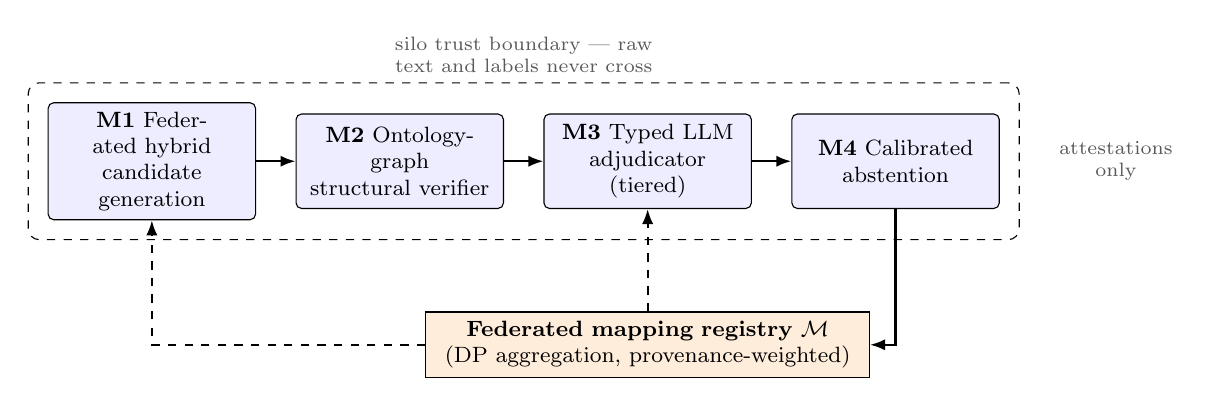
\begin{tikzpicture}[font=\footnotesize,>=Latex,
  mod/.style={draw,rounded corners=2pt,align=center,text width=2.4cm,minimum height=1.2cm,fill=blue!7},
  store/.style={draw,align=center,text width=5.4cm,minimum height=0.75cm,fill=orange!14},
  arr/.style={-{Latex[length=1.9mm]},thick},
  darr/.style={-{Latex[length=1.9mm]},thick,dashed}]
\node[mod] (m1) {\textbf{M1} Federated hybrid\\candidate generation};
\node[mod,right=5mm of m1] (m2) {\textbf{M2} Ontology-graph\\structural verifier};
\node[mod,right=5mm of m2] (m3) {\textbf{M3} Typed LLM\\adjudicator (tiered)};
\node[mod,right=5mm of m3] (m4) {\textbf{M4} Calibrated\\abstention};
\draw[arr] (m1) -- (m2);
\draw[arr] (m2) -- (m3);
\draw[arr] (m3) -- (m4);
\node[store,below=13mm of m3] (reg) {\textbf{Federated mapping registry} $\reg$ \ (DP aggregation, provenance-weighted)};
\draw[arr] (m4.south) |- (reg.east);
\draw[darr] (reg.north) -- (m3.south);
\draw[darr] (reg.west) -| (m1.south);
\begin{scope}[on background layer]
\node[draw,dashed,rounded corners,inner sep=7pt,fit=(m1)(m2)(m3)(m4),
      label={[font=\scriptsize,text=black!65,text width=6.2cm,align=center]above:silo trust boundary --- raw text and labels never cross}] (bound) {};
\end{scope}
\node[font=\scriptsize,align=center,text=black!65,right=4mm of m4,text width=1.9cm] {attestations\\only};
\end{tikzpicture}
\caption{The FedHarm pipeline. Records are embedded locally in M1; only query vectors reach the shared ontology index. M2 types candidates by subsumption and disjointness before any model call. M3 adjudicates residual ambiguity inside the boundary and emits a typed relation with cited evidence. M4 sets the commit set by conformal selection and writes expert-confirmed mappings to the registry, which feeds back into both M1 (fast resolution) and M3 (grounded exemplars), closing the loop.}
\label{fig:arch}
\end{figure*}

\subsection{M1: Federated Hybrid Candidate Generation}

M1 builds, for each record $x$ at site $i$, a candidate set that is deliberately generous, since none of the later stages (M2--M4) can ever add candidates back in, only remove them. Let $G = \{g_{\mathrm{dense}}, g_{\mathrm{lex}}, g_{\mathrm{graph}}, g_{\mathrm{xref}}\}$ be four generators, each returning a ranked list. Then
\begin{equation}
C(x) = \bigcup_{g \in G} C_g(x), \qquad
C_g(x) = \mathrm{top}\text{-}k_g\big(\mathrm{rank}_g(x)\big),
\end{equation}
and each candidate $c$ carries a provenance tag $\mathrm{src}(c) \subseteq G$ recording which generator(s) proposed it.

\begin{itemize}
\item \textbf{Dense retrieval} ($g_{\mathrm{dense}}$) searches a shared index of ontology labels and synonyms using a sentence encoder~\cite{b18}. The record itself is encoded locally at the site; only the resulting vector, possibly clipped and noised, is ever allowed to leave.
\item \textbf{Lexical retrieval} ($g_{\mathrm{lex}}$) uses BM25 over the same index~\cite{b17}. It catches exact-terminology matches that dense encoders sometimes blur together, and its behavior tends to stay stable even as the input distribution shifts.
\item \textbf{Graph expansion} ($g_{\mathrm{graph}}$) takes the strongest lexical and dense hits as starting points and adds their ancestors, descendants, and siblings within a bounded radius $r$ inside $\onto$. This is the generator that turns a near-miss into an actual hit: if the true answer is an ancestor of something already retrieved, plain retrieval will never find it, but one hop of expansion will.
\item \textbf{Cross-reference pivoting} ($g_{\mathrm{xref}}$) follows harvested cross-references through an intermediate vocabulary, the same ICD-10 $\rightarrow$ SNOMED CT $\rightarrow$ MONDO/HPO path used in~\cite{b1}, and it is the only generator that applies when the input records already come pre-coded.
\end{itemize}

Combining all four into a union rather than an intersection is the single most consequential design choice here. The original study found its two generators to be complementary rather than redundant -- only a minority of input codes were caught by both, and neither one alone achieved full coverage~\cite{b1}. Shifting the candidate set from union toward intersection would turn that finding from an observation into a guaranteed architectural property. We should flag right away that our own retrieval pilot on curated alignment tasks does not actually back up combining generators (Section~\ref{sec:pilot}), and we come back later to why that negative result might not carry over from curated terminologies to free clinical text.

\subsection{M2: Ontology-Graph Structural Verifier}

M2 is a symbolic stage. It takes the candidate set and classifies each candidate against an anchor $a(x)$ -- the ontology term already known for $x$, or the one resolved with the most confidence (for coded inputs, the term reached via cross-references; for free text, the highest-scoring lexical-dense agreement). It queries the reasoner to assign
\begin{equation}
\rel\big(a(x), c\big) \in \{\equiv,\ \sqsupseteq,\ \sqsubseteq,\ \bot,\ \sim\},
\end{equation}
where $\bot$ is returned when $\onto \models c \sqsubseteq \neg a(x)$, and $\sim$ is used when the reasoner cannot assert either subsumption or disjointness. Along with the relation, M2 also reports the \emph{specificity direction} (whether $c$ is more generic, more specific, or simply incomparable to the anchor) and the axiom chain that justifies the call, both of which M3 later receives as evidence.

Two things follow from this. First, any candidate typed $\bot$ can be dropped with total certainty: something disjoint from the anchor can never turn out to satisfy an equivalence, broader-than, or narrower-than criterion, so removing it costs nothing for any acceptance relation drawn from $\{\equiv, \sqsupseteq, \sqsubseteq\}$ (Proposition~\ref{prop:prefilter}). Second, for whatever candidates survive, M3 is no longer being asked to guess the relation from raw text; it is being asked to \emph{confirm or refute} a relation the ontology has already asserted or ruled out. This directly targets the biggest source of remaining error in the two-step pipeline, whose mistakes are overwhelmingly confusions of specificity and polarity -- \emph{Grade II} versus \emph{$>$grade 2}, \emph{congenital} versus \emph{acquired}, \emph{APGAR at minute 1} versus \emph{10-minute APGAR}~\cite{b1} -- cases a reasoner resolves exactly and a nearest-neighbour search cannot see at all.

Two independent bodies of evidence support putting this stage first. MILA's retrieve--identify--prompt design arrives at the same principle from the ontology-alignment side, saving model calls only for cases its search genuinely cannot resolve, and reports a 92.6--98.4\% reduction in LLM requests without any loss in quality~\cite{b54}; Proposition~\ref{prop:prefilter} gives a sufficient condition under which that kind of reduction comes at no cost in recall. And the benchmark finding that LLM-only refinement collapses specifically in the biomedical domain -- F1 0.256 for LLMs4OM on SNOMED--FMA versus 0.894 for a matcher-first system on the same task~\cite{b56,b54} -- argues that a structure-aware stage is a requirement, not just a nice-to-have optimization. Worth flagging is an important difference in kind: MILA's structural signal comes from a matcher operating over labels, while M2's comes directly from the ontology's own logical axioms, so the two are complementary rather than doing the same job.

\subsection{M3: Typed LLM Adjudicator}

M3 handles whatever candidates the symbolic stage cannot settle: those typed $\sim$, and those where the structural relation still needs to be checked against the record's actual meaning. It differs from a simple binary yes/no in three ways.

\textbf{Typed output.} The adjudicator returns a structured verdict
\begin{equation}
\big(\hat{r},\ \hat{p},\ \mathcal{E},\ j\big),
\end{equation}
where $\hat{r} \in \mathcal{R}$ is the predicted relation, $\hat{p} \in [0,1]$ is a self-reported confidence, $\mathcal{E}$ is the actual evidence M3 relied on (the M2 axiom chain, the matching label or synonym, the relevant span of the record), and $j$ is a short justification. Requiring evidence citations does two things: it lets a human reviewer check the verdict against the same evidence the model saw, and it gives M4 the feature signal it needs for calibration.

\textbf{In-boundary execution with tiered escalation.} The adjudicator runs on a locally hosted open-weight model, so the record text never has to leave the site. A small local model handles the high-agreement majority of cases; a larger local model is called in only when the small model's score lands in an indeterminate range, or when M2 returned $\sim$ with a conflicting direction, and it resolves whatever is left. Escalation is driven by the score itself, not by a fixed schedule, so cost tracks actual difficulty. This is the architecture's direct answer to the privacy contradiction the original authors raised: the accuracy that comes from a strong validator is preserved, but the validator now sits inside the federation instead of outside it~\cite{b1,b25}.

\textbf{Prompt-configurable criteria.} As in~\cite{b1}, the acceptance criterion is written in plain language, so switching from equivalence to subsumption -- or from ``same or more generic'' to ``same or more specific'' -- is just a configuration change, not a code change. FedHarm keeps this property and adds a machine-readable relation label on top, so the criterion becomes a policy defined over $\mathcal{R}$ rather than a sentence the model has to interpret unaided.

\subsection{M4: Calibrated Abstention and the Federated Mapping Registry}

M4 is the stage that turns individual verdicts into committed mappings and, crucially, into mappings that stick around afterward.

\textbf{Score construction and calibration.} The raw confidence $\hat{p}$ cannot be used directly as a decision score: self-reported LLM confidence is known to be poorly calibrated and usually overconfident~\cite{b19,b28}. So M4 fits a calibration map $\phi$ on a small, per-site labeled calibration set, using temperature scaling or isotonic regression~\cite{b19,b47}, giving
\begin{equation}
s(x,c) = \phi\big(\hat{p}(x,c)\big),
\end{equation}
which can optionally be combined with how well $\hat{r}$ agrees with $\rel(a(x),c)$.

\textbf{Conformal risk control.} Rather than picking $\tau$ by a grid search over a validation split, M4 chooses the largest threshold whose selective risk on the calibration set stays within tolerance, using conformal risk control with a monotone loss~\cite{b22,b23}. This gives the finite-sample guarantee in Proposition~\ref{prop:conformal}, and it directly carries out the constrained objective from Eq.~\eqref{eq:objective}: coverage is maximized subject to a risk cap, and whatever gets deferred becomes the review queue.

\textbf{The registry.} Expert decisions on the deferred residual, together with the high-confidence auto-accepted mappings, get written as \emph{attestations}
\begin{equation}
\alpha = \big(c_{\text{src}},\ c_{\text{tgt}},\ r,\ s,\ \mathrm{prov}\big),
\end{equation}
into the federated mapping registry $\reg$. This registry is aggregated across sites rather than merged without checking: attestation support is counted and weighted by provenance trust and by how well-calibrated the contributing site's own scores tend to be, and the published aggregate has noise added and is suppressed below a support threshold $k_{\min}$, so a mapping attested by fewer than $k_{\min}$ independent sites is never disclosed. This is the point where the architecture introduces a genuine federated-learning problem over the harmonization artifact itself, separate from -- but complementary to -- federated learning over model weights~\cite{b24,b25,b26}. Because a registry entry could reveal that a site holds a record containing a rare local term, the support threshold and the noise scale are part of the disclosure policy from the start, not something bolted on later; we return to this in Section~\ref{sec:analysis}.

\textbf{Closing the loop.} The registry feeds back in two distinct ways, shown in Fig.~\ref{fig:loop}. Used as a \emph{cache}, an attestation resolves any future occurrence of the same source term almost for free, skipping M1--M3 entirely. Used as \emph{grounding}, attested mappings from other sites are retrieved and inserted into M3's context as confirmed precedents, raising adjudication accuracy on the residual cases the cache does not cover. This loop is what makes the architecture cumulative over time: unlike the two-step pipeline, whose output is a dead end, FedHarm's output becomes the next round's input.

\begin{figure}[t]
\centering
\resizebox{\columnwidth}{!}{%
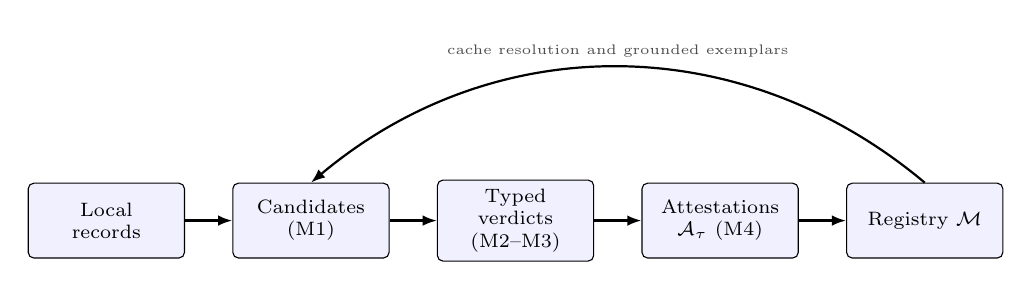
\begin{tikzpicture}[font=\scriptsize,>=Latex,node distance=6mm,
  n/.style={draw,rounded corners=2pt,align=center,text width=1.75cm,minimum height=0.95cm,fill=blue!6},
  arr/.style={-{Latex[length=1.8mm]},thick}]
\node[n] (a) {Local\\records};
\node[n,right=of a] (b) {Candidates\\(M1)};
\node[n,right=of b] (c) {Typed\\
verdicts (M2--M3)};
\node[n,right=of c] (d) {Attestations\\$\att_\tau$ (M4)};
\node[n,right=of d] (e) {Registry $\reg$};
\draw[arr] (a)--(b); \draw[arr] (b)--(c); \draw[arr] (c)--(d); \draw[arr] (d)--(e);
\draw[arr] (e.north) to[out=140,in=40] node[above,font=\tiny,text=black!70,pos=0.5]{cache resolution and grounded exemplars} (b.north);
\end{tikzpicture}}
\caption{The closed loop. Attestations accumulate into a shared registry; the registry both resolves records directly and supplies confirmed precedents to the adjudicator, so coverage compounds across rounds and sites.}
\label{fig:loop}
\end{figure}

\subsection{Operating Modes}

Three modes let the architecture be adopted gradually rather than all at once. In \emph{assisted} mode, M4 auto-accepts nothing at all, and the pipeline simply generates a review queue -- the closest thing to a purely human workflow. In \emph{supervised} mode, the default setting, M4 auto-accepts anything above $\tau$ and routes the rest to experts, while the registry keeps growing in the background. In \emph{autonomous} mode, which only turns on once the registry has saturated for a given ontology pair, unattested records still fall through to M1--M4, but most records get resolved straight from the registry. Because the risk bound is a function of the calibration set and not of the mode itself, moving between modes only changes $\epsilon$ in Eq.~\eqref{eq:objective} -- it does not require changing the architecture.

\section{Evaluation Protocol}
\label{sec:protocol}

We lay out the protocol in detail because the claims this architecture makes are claims about an entire trade-off curve, and a curve cannot be judged from a single point.

\subsection{Datasets and Splits}

Our reference setting is the one established in~\cite{b1}, drawn from the maternal and pediatric therapeutics context of the MPRINT hub~\cite{b37}: a set of unannotated clinical observations covering pregnancy exposures and outcomes, to be mapped onto MONDO and HPO, plus a set of ICD-10-coded outcomes to be mapped onto the same ontologies through an intermediate vocabulary. To actually test the federated claims, records need to be split across simulated sites along a realistic axis -- by institution of origin where that is available, or by a stratification that creates real label-space heterogeneity otherwise, so that different simulated sites genuinely see different concept frequencies. Calibration, registry construction, and evaluation splits must all be kept separate; the registry is never populated using data from the evaluation split.

We also add a second, standardized substrate that the harmonization literature has not used before. The OAEI Bio-ML track supplies curated reference alignments across five ontology pairs -- OMIM--ORDO, NCIT--DOID, SNOMED--FMA, and two SNOMED--NCIT tasks -- with published baselines spanning logic-based, fine-tuned, and LLM-refined systems (Table~\ref{tab:oaei})~\cite{b55,b54}. Running FedHarm on Bio-ML gives two advantages. It makes the architecture directly comparable against a mature literature and a shared reference alignment, rather than against a single expert's private judgment, and it isolates M2's contribution specifically, because Bio-ML's ontology pairs differ sharply in how much structural information they actually expose: aligning SNOMED--FMA leans heavily on subsumption, while NCIT--DOID is mostly a lexical matching problem. If a verifier stack only helps on the structurally rich pairs, that should show up as a clear, task-dependent effect, and we treat that as a testable prediction rather than an assumption. The record-to-ontology setting remains our primary evaluation, since it is the task a real federation actually has to solve; Bio-ML is a controlled add-on, and we report the two separately instead of pooling them together.

\subsection{Reported Performance of Prior Systems}
\label{sec:prior}

Before deciding what to measure ourselves, we lay out what has already been measured by others, because these numbers determine which comparisons are even meaningful. Two distinct task families are at play here, and mixing them up is a common mistake. \emph{Ontology-to-ontology alignment} matches concepts from one ontology against another and is scored against curated reference alignments; \emph{record-to-ontology harmonization} maps patient-derived strings or codes onto ontology terms and is scored against expert judgment. FedHarm addresses the second of these, but the first is where the only standardized benchmark in the field actually lives, and its numbers tell us directly where a verifier stack ought to step in.

Table~\ref{tab:oaei} reports unsupervised results on the OAEI Bio-ML track~\cite{b55}, a machine-learning-friendly biomedical benchmark whose five tasks are built from MONDO and UMLS cross-references. Table~\ref{tab:reported} reports record-to-ontology systems, which use different, non-comparable metrics from one another, so rows should only be compared within the same metric.

\begin{table*}[t]
\caption{Reported performance on the OAEI Bio-ML biomedical ontology-alignment benchmark, unsupervised setting. All values are as published by the original systems and as compiled in~\cite{b54}; none is measured by us. Task difficulty varies widely: OMIM--ORDO is the hardest and NCIT--DOID the easiest.}
\label{tab:oaei}
\centering
\footnotesize
\begin{tabular}{@{}llrrrl@{}}
\toprule
\textbf{System} & \textbf{Task} & \textbf{Precision} & \textbf{Recall} & \textbf{F1} & \textbf{Method family} \\
\midrule
LogMap~\cite{b59}         & OMIM--ORDO            & 0.876 & 0.448 & 0.593 & Logic-based, structure-aware \\
LogMap~\cite{b59}         & NCIT--DOID            & 0.934 & 0.668 & 0.779 & Logic-based, structure-aware \\
BERTMap~\cite{b58}        & OMIM--ORDO            & 0.734 & 0.576 & 0.646 & Fine-tuned encoder \\
BERTMap~\cite{b58}        & NCIT--DOID            & 0.888 & 0.878 & 0.883 & Fine-tuned encoder \\
SORBETMatcher~\cite{b61}  & NCIT--DOID            & 0.920 & 0.907 & 0.913 & Fine-tuned Siamese encoder \\
OLaLa~\cite{b57}          & OMIM--ORDO            & 0.735 & 0.582 & 0.649 & LLM refinement \\
LLMs4OM~\cite{b56}        & OMIM--ORDO            & 0.718 & 0.580 & 0.641 & LLM refinement \\
LLMs4OM~\cite{b56}        & SNOMED--FMA           & 0.211 & 0.326 & 0.256 & LLM refinement (collapses) \\
\midrule
MILA~\cite{b54}           & OMIM--ORDO            & 0.879 & 0.778 & 0.831 & Matcher + LLM for borderline cases \\
MILA~\cite{b54}           & NCIT--DOID            & 0.964 & 0.932 & 0.948 & Matcher + LLM for borderline cases \\
MILA~\cite{b54}           & SNOMED--FMA           & 0.964 & 0.834 & 0.894 & Matcher + LLM for borderline cases \\
MILA~\cite{b54}           & SNOMED--NCIT (Pharm)  & 0.981 & 0.772 & 0.864 & Matcher + LLM for borderline cases \\
MILA~\cite{b54}           & SNOMED--NCIT (Neopl)  & 0.928 & 0.880 & 0.903 & Matcher + LLM for borderline cases \\
\bottomrule
\end{tabular}
\end{table*}

\begin{table*}[t]
\caption{Reported performance of record-to-ontology harmonization systems. Metrics are heterogeneous across rows (expert agreement, accuracy, F1, time reduction) and rows are comparable only within a metric. All values are as published by the cited systems; the final row is our proposed architecture, which is not yet measured and for which we claim no number.}
\label{tab:reported}
\centering
\footnotesize
\begin{tabular}{@{}llll@{}}
\toprule
\textbf{System} & \textbf{Task} & \textbf{Metric} & \textbf{Reported value} \\
\midrule
Kokash et al.~\cite{b1} & MPRINT ICD-10 $\rightarrow$ MONDO/HPO, RAG candidates & Expert agreement & 0.78 \\
Kokash et al.~\cite{b1} & MPRINT ICD-10 $\rightarrow$ MONDO/HPO, SNOMED pivot & Expert agreement & 0.91 \\
Kokash et al.~\cite{b1} & MPRINT unannotated outcomes $\rightarrow$ MONDO/HPO & Expert agreement & 0.92 \\
Kokash et al.~\cite{b1} & Candidate acceptance rate (RAG / SNOMED) & Accepted fraction & 0.423 / 0.147 \\
EHRmonize, GPT-4o 10-shot~\cite{b40} & Medication route abstraction (MIMIC-IV, eICU) & Accuracy & 0.97 \\
EHRmonize, GPT-4o 10-shot~\cite{b40} & Generic drug name extraction & Accuracy & 0.82 \\
EHRmonize, GPT-4o 10-shot~\cite{b40} & Antibiotic binary classification & F1 & 1.00 \\
EHRmonize~\cite{b40} & Annotation time versus fully manual review & Reduction & 60.4--67.9\% \\
MILA~\cite{b54} & LLM requests versus baseline retrieve-then-prompt & Reduction & 92.6--98.4\% \\
\midrule
FedHarm (this work) & Record-to-ontology harmonization, federated & --- & not measured \\
\bottomrule
\end{tabular}
\end{table*}

Three conclusions follow from these tables, and each one directly shapes the design decisions in Sections~\ref{sec:arch} and \ref{sec:protocol}.

\textbf{(i) Adjudication, not retrieval, is where accuracy actually gets lost.} On the Bio-ML benchmark, candidate retrieval recovers up to 100\% of the reference mappings, yet end-to-end performance falls by up to 30\% once prompting enters the picture -- and by up to 50\% specifically in the biomedical domain, where LLM-based refinement performs worst~\cite{b54}. The SNOMED--FMA row in Table~\ref{tab:oaei} makes this especially clear: a purely LLM-refined system reaches only F1 0.256~\cite{b56}, where a matcher-plus-borderline-LLM system reaches 0.894 on the exact same task~\cite{b54}. A pipeline that treats the language model as the sole decision-maker is not just imprecise, then; it throws away most of the recall its own retrieval step already earned. This is the empirical justification for placing a symbolic stage ahead of adjudication (M2), and it is why we treat the LLM as one layer of a verifier stack rather than as the validator by itself.

\textbf{(ii) Saving the model for hard cases keeps quality up and removes most of the cost.} MILA's retrieve--identify--prompt design makes exactly this move on the alignment side, and it reports a 92.6--98.4\% reduction in LLM requests compared with a baseline retrieve-then-prompt pipeline, while still leading on four of five tasks~\cite{b54}. Proposition~\ref{prop:prefilter} explains why a reduction of this size can come without a corresponding drop in recall. The original harmonization pipeline does not take advantage of this, because its adjudicator gets called on every single candidate all four of its generators produce.

\textbf{(iii) Expert effort, not model accuracy, is the quantity that actually determines scale.} EHRmonize cuts annotation time by 60.4--67.9\% compared with fully manual labeling while still keeping a clinician in the loop, and it reports the residual corrections needed as a small, countable set~\cite{b40}. This is a direct precedent for treating review burden as something worth reporting in its own right, not as an implementation detail, and it is why Section~\ref{sec:protocol} measures coverage at a fixed error tolerance instead of accuracy at full coverage. The harmonization systems in Table~\ref{tab:reported} each report a single operating point; the alignment systems in Table~\ref{tab:oaei} report precision, recall, and F1 at full coverage. Neither kind reports a full risk--coverage curve, which means neither one actually states the error rate a real deployment would face at a chosen level of automation.

\subsection{Baselines and Ablations}

\begin{itemize}
\item \textbf{B1, retrieval only.} M1's candidate generators with no validation at all -- essentially the source pipeline's Step~1~\cite{b1}. This establishes the ceiling on recall.
\item \textbf{B2, two-step pipeline.} M1 plus a binary LLM adjudicator, using the published prompt~\cite{b1}. This is the direct point of comparison.
\item \textbf{B3, union retrieval + binary LLM.} B2, but with M1's multi-generator union, so we can separate what wider candidate coverage buys from what the verifier stack buys.
\item \textbf{B4, FedHarm without M2.} The full pipeline minus the structural verifier, isolating the symbolic stage's contribution.
\item \textbf{B5, FedHarm without M4 calibration.} Abstention decided by raw self-reported confidence and a fixed threshold, isolating what calibration adds.
\item \textbf{B6, FedHarm without the registry.} The loop left open, isolating the effect of reuse.
\end{itemize}
The full architecture is evaluated in all three operating modes. A factorial ablation crossing \{M2 on/off\} $\times$ \{M4 on/off\} $\times$ \{registry on/off\} separates each module's individual effect from any interaction between them, which matters because the original study found that components can interact non-additively -- a single change can help in isolation but hurt when combined with others -- and we expect the same to be true of a verifier stack~\cite{b1}.

\subsection{Metrics}

\begin{itemize}
\item \textbf{Mapping quality.} Precision, recall, and F1 of committed mappings, calculated separately for each relation class, since a pipeline that is reliable for $\equiv$ might not be reliable for $\sqsubseteq$.
\item \textbf{Risk--coverage.} The curve $\mathrm{cov}(\tau) \mapsto \mathrm{risk}(\tau)$, summarized by the area under the risk--coverage curve and by precision at fixed coverage levels (50\%, 70\%, 90\%). This is our primary metric; a single precision number at full coverage, the kind the two-step pipeline reports, is just the $\mathrm{cov}=1$ endpoint of this curve and the least informative point on it.
\item \textbf{Automation coverage at risk tolerance.} The largest coverage that still satisfies the error-rate bound for $\epsilon \in \{0.05, 0.10, 0.20\}$: for FedHarm, this is the accepted-set size under the Benjamini--Hochberg rule from Proposition~\ref{prop:conformal}, together with the empirical false discovery rate measured against the nominal $\epsilon$; for threshold baselines, it is simply the largest $\mathrm{cov}(\tau)$ with $\mathrm{risk}(\tau) \le \epsilon$. The gap between the nominal and empirical error rate is reported as its own column, since it is the direct test of whether calibration is actually working.
\item \textbf{Review burden.} The fraction of candidates routed to expert review under M4, compared against a baseline where every candidate gets reviewed; reported per site. EHRmonize's 60.4--67.9\% reduction in annotation time under mandatory clinician oversight is the closest published precedent, and it sets the bar this metric should be measured against~\cite{b40}, though time reduction and the fraction of candidates reviewed are different quantities, so we report both.
\item \textbf{Reuse and transfer.} The registry's hit rate over successive rounds; the share of a site's records that get resolved by a cache entry attested at \emph{another} site, which is our measure of cross-site harmonization transfer.
\item \textbf{Privacy--utility.} Mapping quality and registry hit rate as functions of the privacy budget and support threshold, with the guarantee certified using an accounting method suited to whatever noising scheme is in use~\cite{b24}.
\item \textbf{Cost.} Adjudicator calls per record, split between tier-1 and tier-2, along with wall-clock time and token cost per committed mapping, so the symbolic stage's savings can be measured rather than just claimed.
\end{itemize}

\subsection{Expert Protocol and Statistical Analysis}

The original study measured agreement against a single expert, which it correctly flags as a limitation of its own design, and it also found that a single expert's judgments can shift once the acceptance criterion is clarified~\cite{b1}. Because of this, our protocol calls for a panel of at least three clinical reviewers, each with their own disjoint subset of cases plus a shared subset used to measure inter-annotator agreement, with the relation criterion fixed in writing before annotation ever starts. Agreement is reported using Cohen's $\kappa$ or Krippendorff's $\alpha$ among the experts themselves, and expert-versus-architecture agreement is reported against the panel's majority verdict, with the panel's own disagreement rate serving as a natural ceiling. Comparisons across baselines use paired bootstrap resampling over records, with confidence intervals; since the baselines all share the same candidates, a paired design is both more statistically powerful and a more honest comparison than simply comparing marginal accuracy numbers against each other.

\subsection{Reporting Format and Published Baselines}

Table~\ref{tab:results} fixes the reporting format in advance and pre-fills the two baseline rows with the original study's published values, so that the anchor for comparison is stated outright rather than left implicit~\cite{b1}. Anything a reviewer would otherwise have to take on faith is confined strictly to the baseline block and clearly marked as such; nothing in the rows we are responsible for is an estimate. Every FedHarm row in this table is still left empty, because none of them have been run on the MPRINT reference setting or its exact metric definitions. A full-pipeline measurement does now exist -- on a different substrate, the two public Bio-ML tasks, with a bounded sample size and idealized expert review -- and is reported in full in Section~\ref{sec:fullpilot}; we do not fold those numbers into this table because doing so would mix two different candidate distributions and evaluation protocols under one set of column headers, which is exactly the kind of comparison Section~\ref{sec:prior} warns against.

\begin{table*}[t]
\caption{Evaluation table for FedHarm. The B1--B2 rows reproduce values published by the source study~\cite{b1} and are \emph{not} our measurements; the remaining rows are to be produced by the protocol of this section and are reported as empty rather than estimated. ``---'' denotes a quantity the source does not report. Precision for B2 is the expert-agreement rate, which that study also reports as mapping precision.}
\label{tab:results}
\centering
\footnotesize
\begin{tabular}{@{}llrrrrr@{}}
\toprule
\textbf{Method} & \textbf{Candidate generation} & \textbf{Precision} & \textbf{Recall} & \textbf{Coverage at $\epsilon$} & \textbf{Emp.\ FDR} & \textbf{Reuse} \\
\midrule
\multicolumn{7}{@{}l}{\textit{Prior systems --- values as published by~\cite{b1}, not measured by us}} \\
B1 Retrieval only~\cite{b1}     & RAG, $k{=}3$      & --- & 0.98\textsuperscript{a} & --- & --- & --- \\
B1 Retrieval only~\cite{b1}     & SNOMED pivot      & --- & 0.688\textsuperscript{b} & --- & --- & --- \\
B2 Two-step pipeline~\cite{b1}  & RAG, $k{=}3$      & 0.78 & --- & --- & --- & 0.00 \\
B2 Two-step pipeline~\cite{b1}  & SNOMED pivot      & 0.91 & --- & --- & --- & 0.00 \\
B2 Two-step pipeline~\cite{b1}  & Unannotated, $k{=}3$ & 0.92 & --- & --- & --- & 0.00 \\
\midrule
\multicolumn{7}{@{}l}{\textit{Our systems --- to be produced by the protocol of Section~\ref{sec:protocol}}} \\
B3 Union + binary LLM           & union of four generators & \TBD & \TBD & \TBD & \TBD & 0.00 \\
B4 FedHarm without M2           & union, no structural verifier & \TBD & \TBD & \TBD & \TBD & \TBD \\
B5 FedHarm without calibration  & union, M2, uncalibrated LLM & \TBD & \TBD & \TBD & \TBD & \TBD \\
B6 FedHarm without registry     & full, loop open & \TBD & \TBD & \TBD & \TBD & 0.00 \\
FedHarm (supervised)            & full pipeline & \TBD & \TBD & \TBD & \TBD & \TBD \\
FedHarm (autonomous)            & full, saturated registry & \TBD & \TBD & \TBD & \TBD & \TBD \\
\bottomrule
\end{tabular}

\smallskip
{\footnotesize \textsuperscript{a}Ceiling the source reports would be attainable by expanding retrieval to $k{=}10$ (98\% of entries); it is not a measured end-to-end recall. \textsuperscript{b}Derived by us from a published count: 800 of 1{,}162 ICD-10 codes yielded at least one candidate.}
\end{table*}

\subsection{Pre-registered Targets and Their Anchors}
\label{sec:targets}

We state in advance what would actually count as success, and every target is anchored to a number another system has already published, not to a value chosen for convenience. Table~\ref{tab:targets} is the numeric companion to Table~\ref{tab:results}: it gives the benchmark each cell needs to be measured against. Every value in its anchor column belongs to another system's published result, never to ours; the fourth column reports what we actually measured in the pilot of Section~\ref{sec:fullpilot}, where applicable -- T1 and T4 require ablations (B3, B4) we have not yet run, and are left untested.

\begin{table}[t]
\caption{Pre-registered targets for FedHarm, the published results that anchor them, and what the bounded pilot (Section~\ref{sec:fullpilot}) actually measured. ``---'' means no published analogue exists (T6) or the ablation needed to test the target has not been run (T1, T4).}
\label{tab:targets}
\centering
\footnotesize
\begin{tabular}{@{}p{0.6cm}p{1.85cm}p{2.55cm}p{2.6cm}@{}}
\toprule
\textbf{ID} & \textbf{Target} & \textbf{Anchor} & \textbf{Measured (pilot)} \\
\midrule
T1 & $\ge$80\% fewer adjudicator calls than B3 & 92.6--98.4\% fewer LLM requests, OAEI~\cite{b54} & Not tested (no B3 ablation run) \\
T2 & FDR $\le$ 0.10 at coverage $\ge$ 0.70 & Source commits to 100\% at precision 0.78--0.92~\cite{b1} & \emph{Not met}: coverage $=0$ at $\epsilon\in\{0.05,0.10,0.20\}$ on both tasks -- raw LLM confidence too weakly separated to license any auto-accept \\
T3 & B3 recall exceeds B2 recall & Union gained 0.004/0.000 recall on Bio-ML~\cite{b1} & \emph{Tested; not supported} -- same result, reconfirmed \\
T4 & B4 FDR rises in specificity/polarity classes & F1 0.256 vs.\ 0.894, SNOMED--FMA~\cite{b56,b54} & Not tested (no B4 ablation run) \\
T5 & Review fraction $\le$ 0.30 & 60.4--67.9\% time reduction~\cite{b40} & \emph{Not met}: review fraction $=1.00$ at every tested $\epsilon$ (follows directly from T2) \\
T6 & Registry reuse $\ge$ 0.40 by round three & ---\ (monotonicity from Prop.~\ref{prop:registry}) & \emph{Not met at pilot scale}: cumulative hit rate $\approx$1\% by round three on NCIT--DOID and 0\% on OMIM--ORDO, though registry size itself grows monotonically every round on both tasks \\
\bottomrule
\end{tabular}
\end{table}

Three of these targets are now falsifiable in a strong sense and have been tested. T3 fails outright if combining generators does not raise recall above what a single generator achieves; it was testable without any language model, and the pilot in Section~\ref{sec:pilot} does not support it. T2 and T5 are linked: T5's review-fraction target can only be met if T2's coverage target is met first, and neither was, because the pilot's calibration signal (raw self-reported LLM confidence) carries almost no information about correctness (Section~\ref{sec:fullpilot}). T6 is also not met at this pilot's scale, but for a different reason -- it is a small-sample and short-horizon artifact of a synthetic recurrence probability applied to only 70 queries per task, not evidence against Proposition~\ref{prop:registry}'s monotonicity claim, which held exactly as proved in every round we ran. T1 and T4 remain untested because they require ablations (removing the structural verifier or comparing against a non-verifier baseline) that this pilot did not run. Table~\ref{tab:targets} was written as a commitment about how comparisons would be made, not a forecast of results, and we are reporting against that commitment rather than revising it after the fact.

\section{Analytical Properties}
\label{sec:analysis}

The architecture supports four claims that hold regardless of any experiment.

\begin{proposition}[Structural pre-filtering is lossless for the acceptance relation]
\label{prop:prefilter}
Let $\mathcal{R}^{+} \subseteq \{\equiv, \sqsupseteq, \sqsubseteq\}$ be the set of relations the acceptance criterion admits, let $C(x)$ be the candidate set, and let $\tilde{C}(x) = \{c \in C(x) : \rel(a(x),c) \neq \bot\}$ be the set surviving M2, where $\rel$ is computed by a sound reasoner. Then no candidate whose true relation to the anchor lies in $\mathcal{R}^{+}$ is removed, and $|\tilde{C}(x)| \le |C(x)|$, with equality if and only if no candidate is disjoint from the anchor.
\end{proposition}

\noindent\textit{Proof.} Suppose $\rel(a(x),c) = \bot$, so $\onto \models c \sqsubseteq \neg a(x)$. Since $a(x)$ and $c$ are satisfiable ontology terms, it follows that $c$ is disjoint from $a(x)$, hence can be neither equivalent to it, nor broader, nor narrower than it. The true relation of $c$ therefore cannot lie in $\mathcal{R}^{+}$, so removal discards no admissible candidate. The cardinality claim is immediate. \hfill$\square$

In plain terms, this proposition is what justifies putting a cheap, exact stage ahead of an expensive, approximate one: M2 can never remove more candidates than it should, and every candidate it does remove is one whose apparent similarity was only ever coincidental.

\begin{proposition}[Finite-sample control of the accepted-set error rate]
\label{prop:conformal}
For a candidate $(x,c)$ let $H(x,c)$ be the null hypothesis that its true relation does not lie in $\mathcal{R}^{+}$, and let $p(x,c) \in (0,1]$ be a conformal p-value for $H(x,c)$ computed against a calibration set exchangeable with the test population~\cite{b50,b52}. Let $\att_\epsilon$ be the set of candidates selected by the Benjamini--Hochberg rule at level $\epsilon$ applied to the test p-values. Then
\begin{equation}
\mathrm{FDR}(\att_\epsilon)
\;=\;
\mathbb{E}\!\left[
\frac{\big|\{(x,c) \in \att_\epsilon : H(x,c)\ \text{holds}\}\big|}{\max\{|\att_\epsilon|,1\}}
\right]
\;\le\; \epsilon ,
\end{equation}
and, under independence of the p-values, $\att_\epsilon$ is the largest threshold rule satisfying that bound.
\end{proposition}

\noindent\textit{Proof.} Conformal p-values are super-uniform under the null whenever calibration and test candidates are exchangeable~\cite{b50}, which is exactly the validity condition the Benjamini--Hochberg procedure requires. The procedure's theorem then yields $\mathrm{FDR} \le \epsilon$ for positively dependent p-values and, under independence, identifies it as the largest threshold set with that property~\cite{b53}. \hfill$\square$

In practical terms, Proposition~\ref{prop:conformal} is what lets us say that M4 turns an uncalibrated model score into a contract that can actually be deployed. It also explains why the original pipeline's reported precision range cannot be acted on directly: a precision number without a matching coverage number and a calibrated score is just one point on a curve that was never measured. Two qualifications matter enough to state up front rather than bury in a footnote. First, the quantity actually being controlled here is the false discovery rate -- the error rate of the accepted set, averaged over selections; if a bound on the expected fraction of errors across \emph{all} candidates is what is wanted instead, the conformal risk control construction from~\cite{b22} can be used, at the cost of an operating point that is somewhat less directly interpretable. Second, this guarantee is distribution-free, but it is not assumption-free: it requires exchangeability, a condition a site with unusual coding practices might well violate. A simple accept/reject pipeline reports neither of these quantities.

\begin{proposition}[Registry coverage is monotone under accept-only retention]
\label{prop:registry}
Let $\reg_t$ be the registry after round $t$, and let $R_t$ be the fraction of records resolved directly from $\reg_t$. If the retention rule is accept-only---an attestation, once published, is never revoked or overwritten---and registry lookup is deterministic, then $R_t \le R_{t+1}$ for all $t$.
\end{proposition}

\noindent\textit{Proof.} Accept-only retention gives $\reg_t \subseteq \reg_{t+1}$, so the set of source terms for which a registry entry exists grows. The resolved set satisfies $\{x : \reg_t(x) \neq \bot\} \subseteq \{x : \reg_{t+1}(x) \neq \bot\}$, whence $R_t \le R_{t+1}$. \hfill$\square$

This holds only under accept-only retention, and it is exactly what revocation, provenance decay, or DP suppression below $k_{\min}$ can undo -- which is why we state the condition explicitly instead of claiming the result unconditionally. In practice, it means that as long as the loop stays stable, it accumulates cleanly over time: the amortized cost of harmonization drops as a consortium grows in size and a study runs longer, which is exactly what turns "a reusable library" from a wish into a built-in architectural consequence.

\begin{proposition}[Boundary-independent communication cost]
\label{prop:comm}
Per round, site $i$ transmits $|\att_i|$ attestations of constant size, so the architecture's communication is $O\!\left(\sum_i |\att_i|\right)$, independent of $|D_i|$, of the number of records adjudicated, and of any embedding dimension used inside the boundary.
\end{proposition}

\noindent\textit{Proof.} The only objects crossing the boundary are query vectors---fixed-length, independent of $|D_i|$---and attestations, each a tuple of two ontology identifiers, a relation label, a scalar score, and provenance metadata. Registries are broadcast once and cached. No term proportional to local dataset size or record length appears in either direction. \hfill$\square$

This is the property that makes the design a federated one in the strict sense, rather than merely a distributed one: how much traffic crosses the boundary depends on the \emph{harmonization artifact} itself, not on how much data is being harmonized.

\subsection{Privacy and Adversarial Surface of the Registry}

Adding a shared artifact also adds a shared attack surface, and we treat that as part of the architecture rather than as an afterthought. Two risks matter here.

\textbf{Inference from attestations.} A published mapping from a rare local term to an ontology code can reveal that a site holds at least one record containing that term. The standard mitigations are the ones we build in from the start: the support threshold $k_{\min}$ suppresses mappings attested by too few independent sites, and calibrated noise bounds how much any single attestation can disclose~\cite{b24,b25}. Since the registry gets queried repeatedly over the life of a study, the combined effect of these many releases has to be accounted for -- not just the privacy of any one release in isolation.

\textbf{Poisoning by a participating site.} A malicious or simply broken site can attest to mappings that are wrong, and a naive majority-rule scheme in a small consortium can be swayed by even one bad-faith participant. The architecture's defenses here are structural rather than relying on trust: provenance-weighted aggregation down-weights sites whose attestations later turn out to be contradicted by expert review, and robust aggregation rules originally developed for Byzantine-tolerant federated learning -- trimmed means, distance-based filtering -- apply directly here as well, since attestation aggregation is really just aggregating a finite multiset of labels with numeric scores~\cite{b51}. It is also worth noting that the adversarial surface is smaller than it first looks: M2 stays sound no matter what any site attests, so a poisoned registry can degrade the cache but cannot make a genuinely disjoint candidate become acceptable, and the conformal guarantee is computed over each site's own calibration set, not over the shared registry.

\subsection{Where the Architecture Can Still Fail}

Three failure modes are foreseeable and deserve to be measured rather than argued away. First, if the anchor $a(x)$ used in M2 is itself wrong -- which happens when the record is unannotated and the top lexical-dense agreement turns out to be mistaken -- then structural typing simply propagates that error forward, and the pre-filter stops being lossless with respect to the \emph{true} relation. M2's soundness is only ever relative to the anchor, so the protocol needs to report anchor accuracy as its own, separate number. Second, the conformal guarantee needs exchangeability between calibration and test data, something a new site with different coding practices can violate; in that case the guarantee only holds conditionally, and coverage should be re-estimated separately for each site. Third, a registry that saturates on easy concepts can lock in a wrong mapping that was attested early on and never revisited afterward; accept-only retention, the very thing that gives us Proposition~\ref{prop:registry}, is what makes this possible, and a carefully controlled revocation policy is the price of being able to fix it later.

\section{Measured Pilot on Bio-ML}
\label{sec:pilot}

\subsection{Retrieval-Only Pilot (M1)}
\label{sec:pilot-m1}

\begin{figure*}[t]
\centering
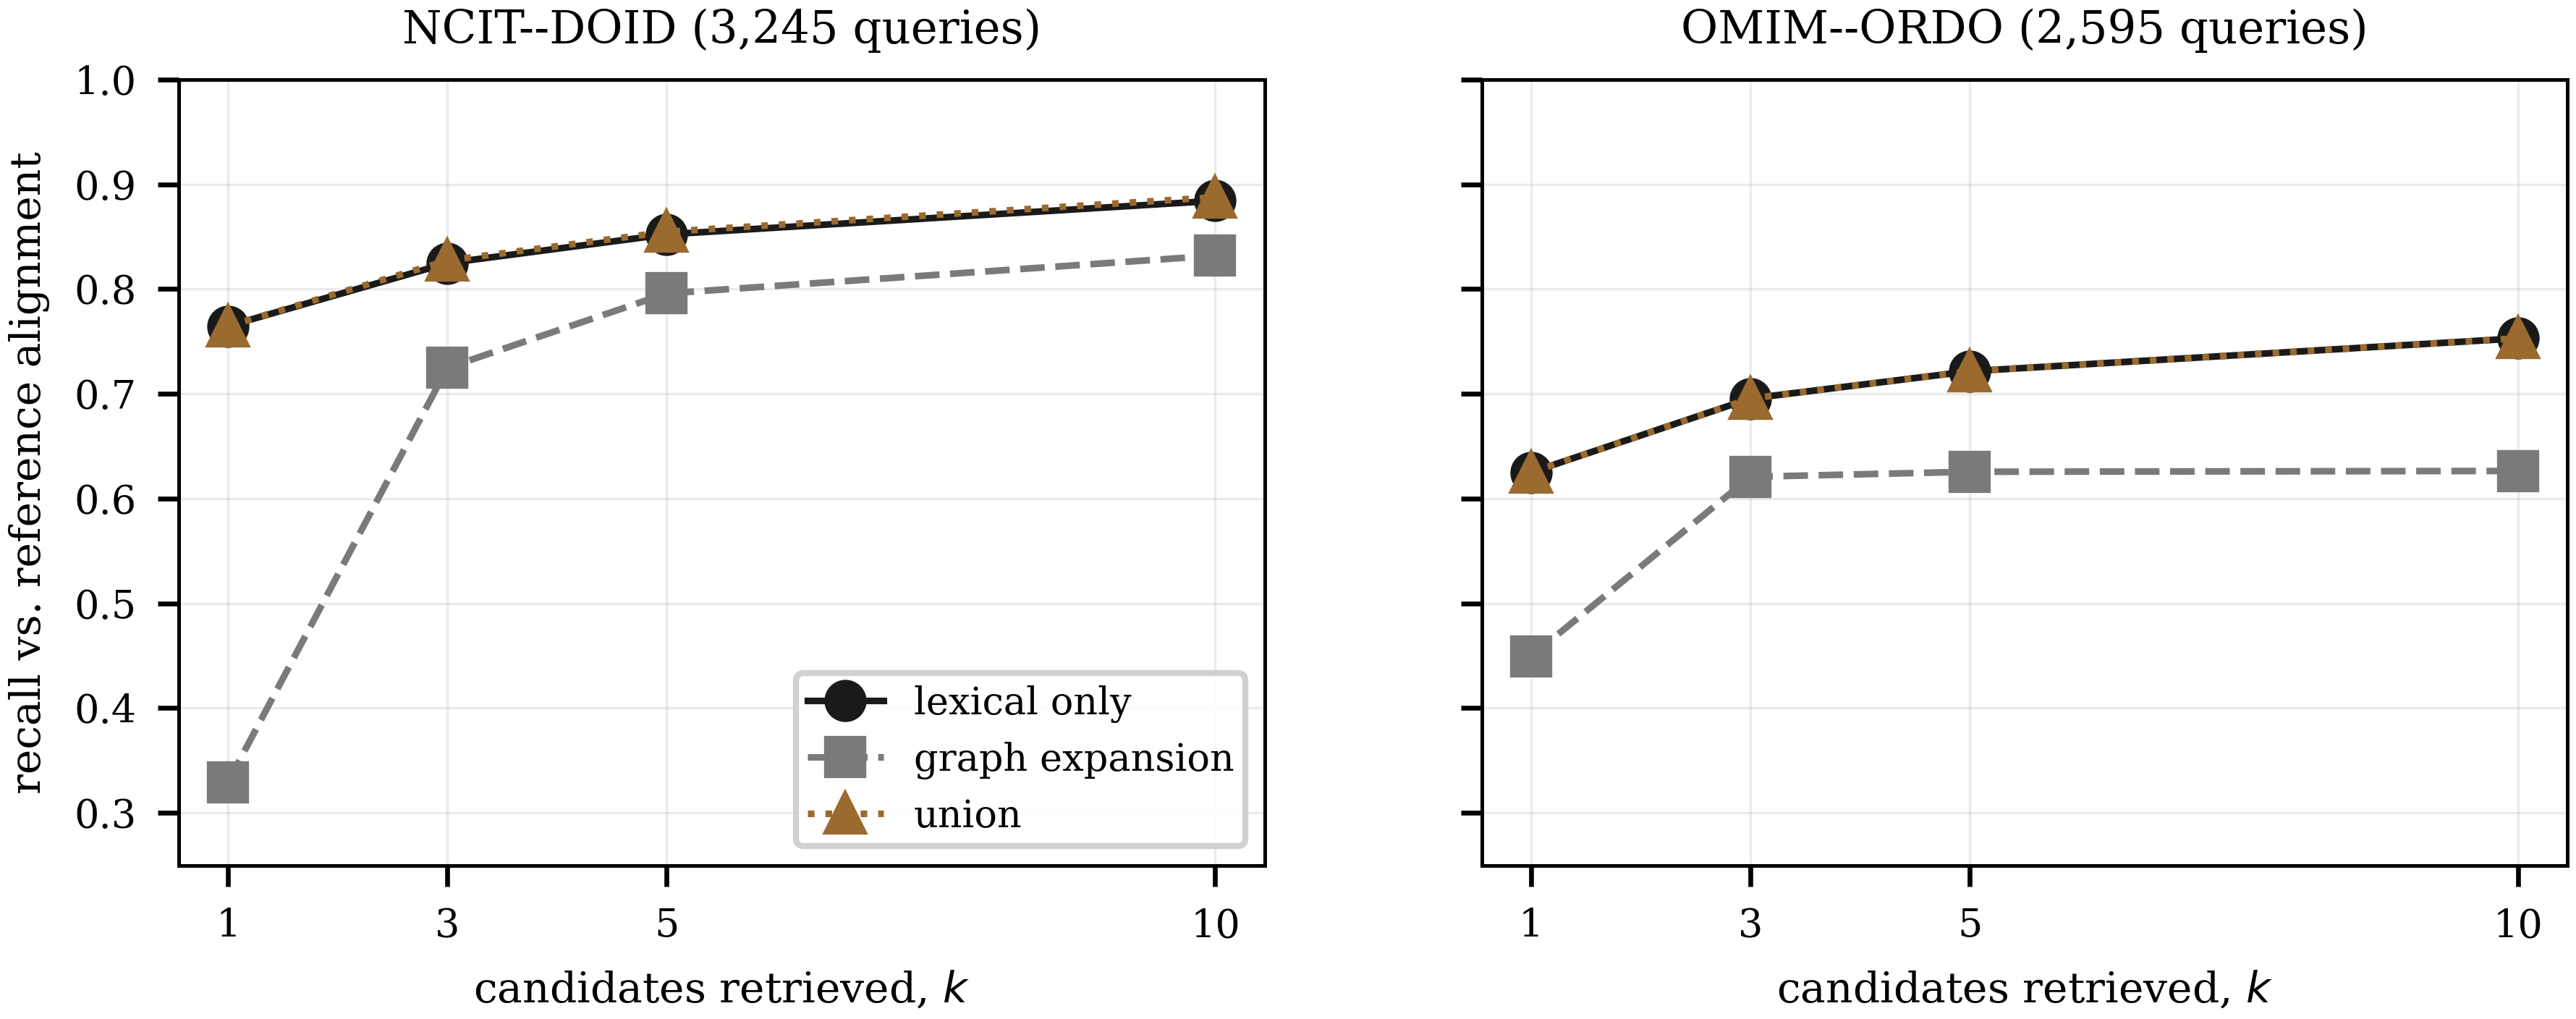
\includegraphics[width=\textwidth]{figs/fig_recall_k.png}
\caption{Recall against number of retrieved candidates, measured on the two openly licensed Bio-ML tasks. The union curve is visually coincident with the lexical curve at every $k$ on both tasks, which is the negative result reported below: adding the graph generator changes recall by at most 0.004 while inflating the candidate set by 23--45\%. On OMIM--ORDO the graph generator is the weakest of the three throughout.}
\label{fig:recallk}
\end{figure*}

The only part of FedHarm that can be run without a language model is M1, and we report the outcome even though it works against one of our own pre-registered predictions. The pilot covers the two Bio-ML tasks built on openly licensed ontologies -- NCIT--DOID and OMIM--ORDO -- and leaves out the three SNOMED-based tasks, which require a license we do not have. It implements one of M1's four generators: BM25 lexical retrieval over target labels and synonyms, tested against the reference equivalence alignments. A second generator that expands the asserted class hierarchy around the leading lexical anchors is implemented in two variants, one limited to parents and children of the top anchor and one expanding siblings from the top three anchors. Dense retrieval needs an encoder we did not have access to, and cross-reference pivoting needs SNOMED CT. This retrieval-only measurement therefore tests only M1's candidate-generation claim (T3 below); Section~\ref{sec:fullpilot} reports a separate, full-pipeline pilot that does exercise M2, M3, and M4 together, on a smaller query sample, and neither pilot fills in Table~\ref{tab:results}, which is scoped to the MPRINT reference setting.

\begin{table*}[t]
\caption{Measured retrieval pilot on the OAEI Bio-ML benchmark. Values are our own measurements against the reference equivalence alignments; candidate counts are means over queries. The union row is the bounded expansion variant, which is the more favourable of the two we tried.}
\label{tab:pilot}
\centering
\footnotesize
\begin{tabular}{@{}llrrrr@{}}
\toprule
\textbf{Task (\#queries)} & \textbf{Generator} & \textbf{P} & \textbf{R} & \textbf{F1} & \textbf{Cand.} \\
\midrule
NCIT--DOID (3{,}245) & lexical, $k{=}1$  & 0.769 & 0.765 & 0.766 & 9.0 \\
NCIT--DOID           & lexical, $k{=}10$ & 0.148 & 0.884 & 0.221 & 9.0 \\
NCIT--DOID           & graph, $k{=}10$   & 0.324 & 0.829 & 0.451 & 4.2 \\
NCIT--DOID           & union, $k{=}10$   & 0.116 & 0.888 & 0.197 & 11.1 \\
\midrule
OMIM--ORDO (2{,}595) & lexical, $k{=}1$  & 0.626 & 0.625 & 0.625 & 9.6 \\
OMIM--ORDO           & lexical, $k{=}10$ & 0.100 & 0.753 & 0.162 & 9.6 \\
OMIM--ORDO           & graph, $k{=}10$   & 0.307 & 0.626 & 0.411 & 5.4 \\
OMIM--ORDO           & union, $k{=}10$   & 0.087 & 0.753 & 0.152 & 13.9 \\
\bottomrule
\end{tabular}
\end{table*}

Two observations come out of this, and the second one goes against a claim we made earlier.

\textbf{(i) Lexical retrieval alone already works well on curated terminologies.} A single BM25 generator over labels and synonyms reaches $F_1 = 0.766$ at rank one on NCIT--DOID and 0.625 on OMIM--ORDO, with recall climbing to 0.884 and 0.753 once ten candidates are allowed. This matches what the alignment literature has already found -- that lexical information alone is the single most successful source for biomedical matching~\cite{b59,b60} -- and it is why NCIT--DOID is considered the easier of the two Bio-ML tasks. Fig.~\ref{fig:recallk} shows the recall curves, and Fig.~\ref{fig:prplane} places this generator in the precision--recall plane alongside the published systems from Table~\ref{tab:oaei}.

\begin{figure}[t]
\centering
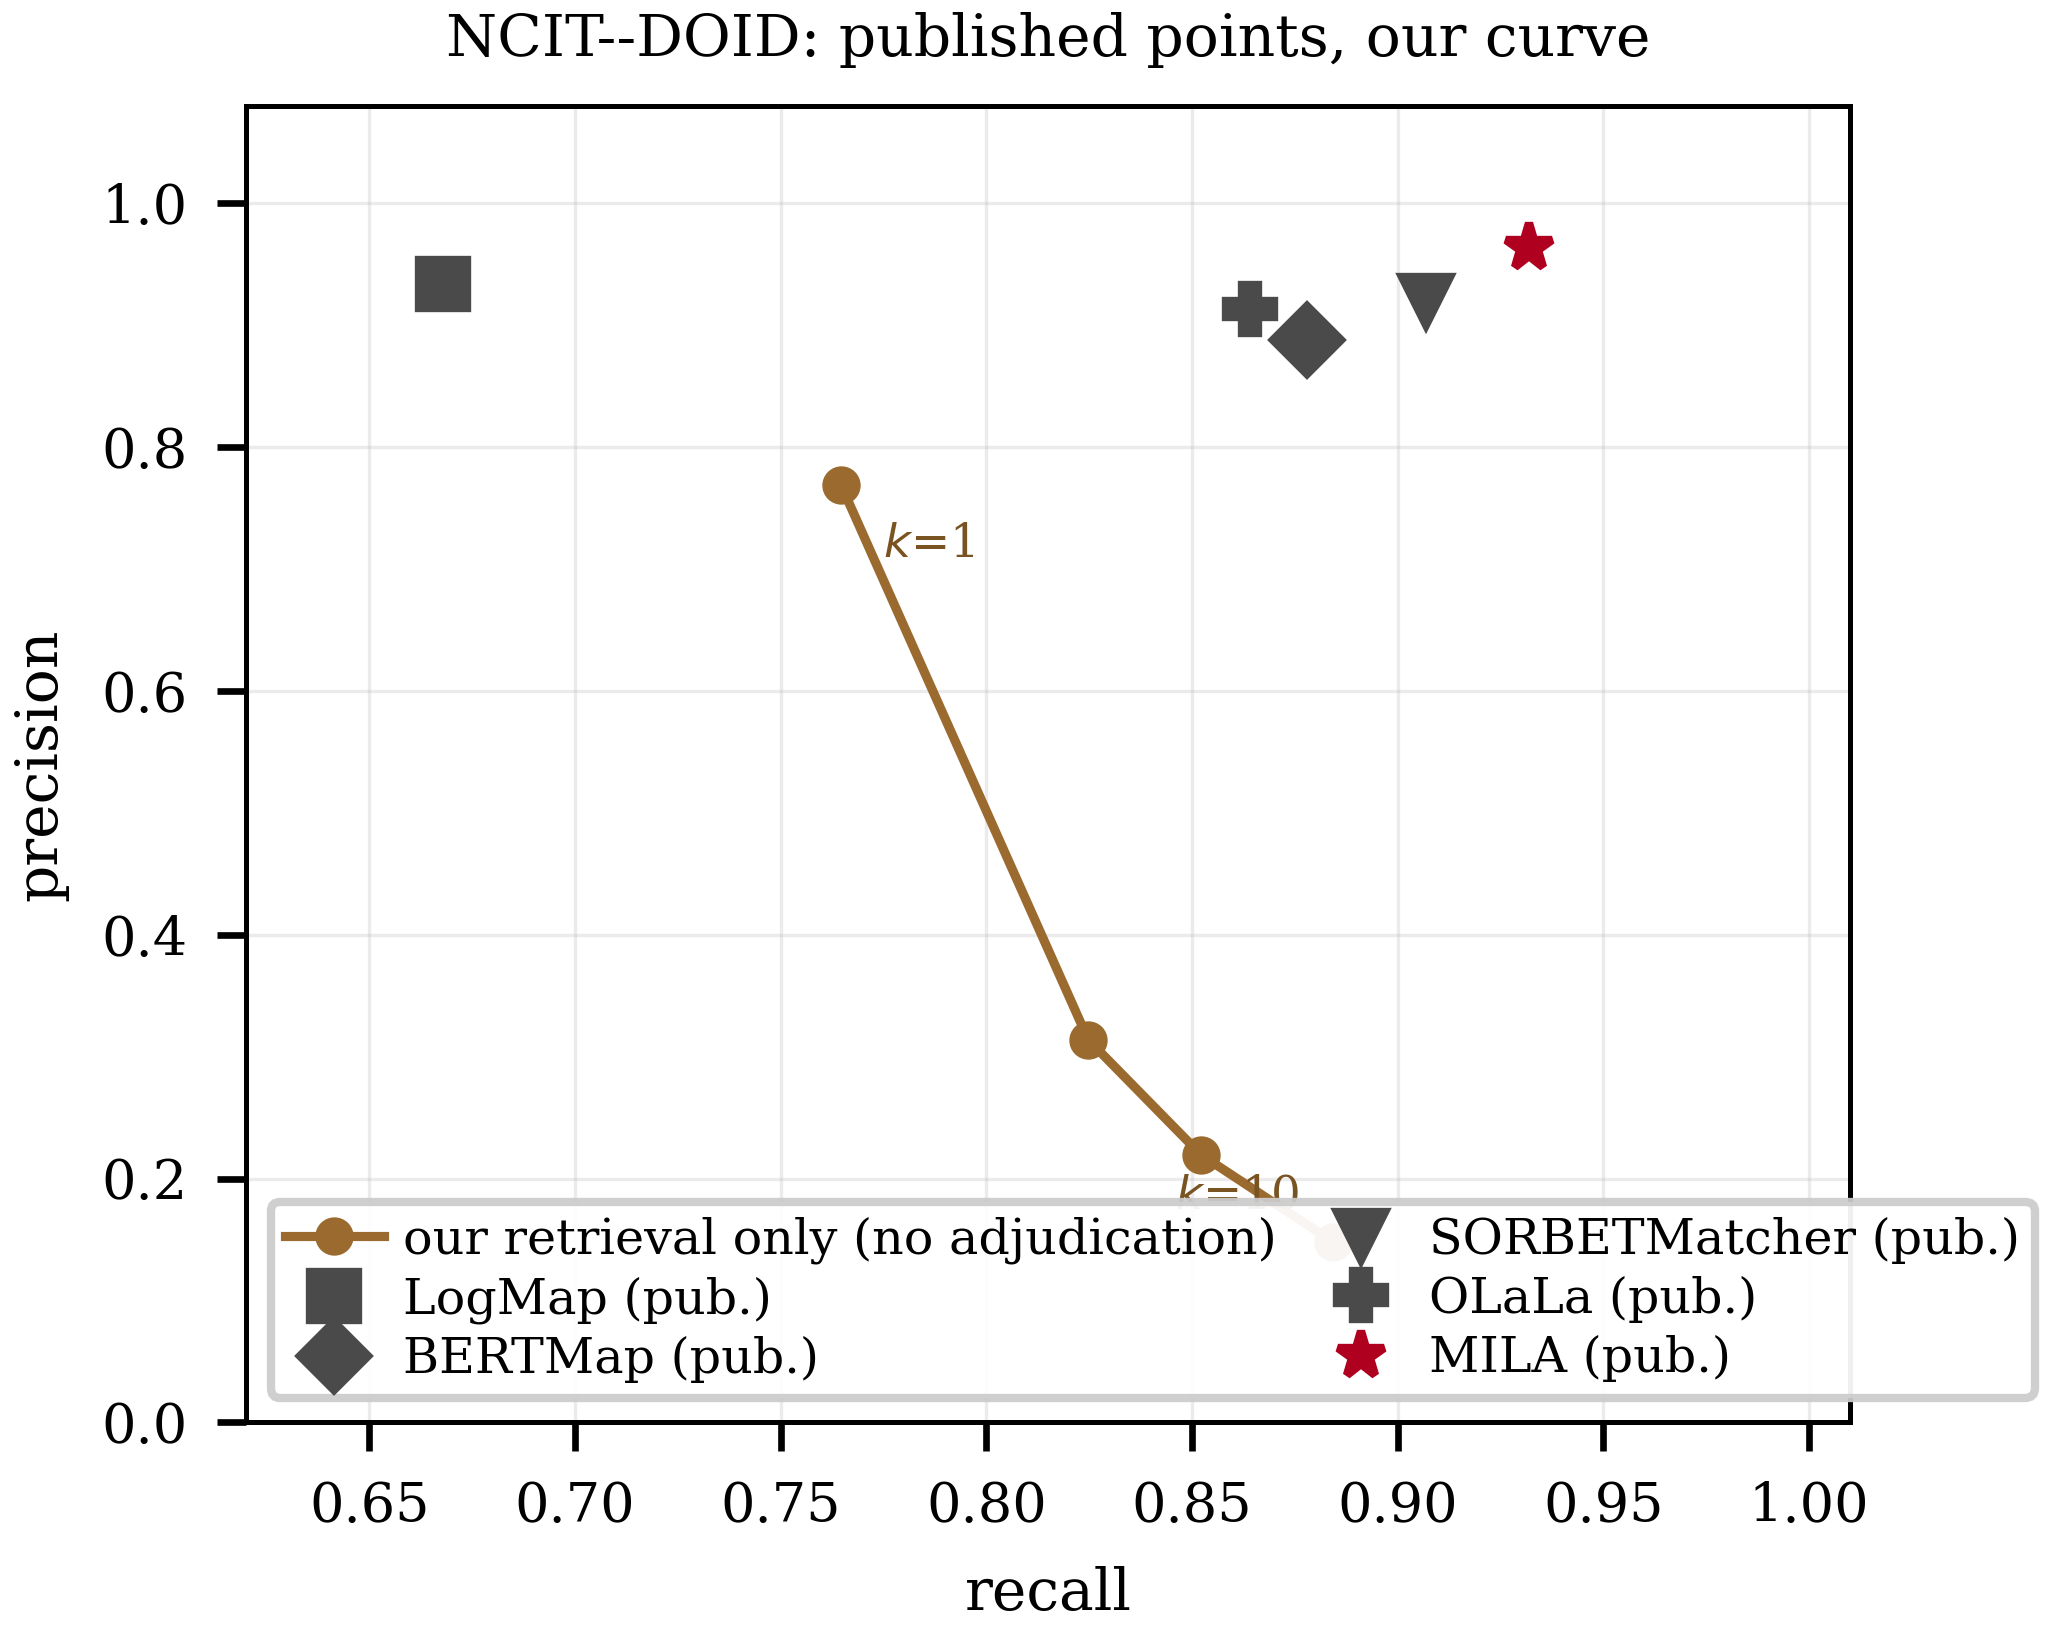
\includegraphics[width=\columnwidth]{figs/fig_pr_plane.png}
\caption{NCIT--DOID in the precision--recall plane. Published systems report a single operating point each, because they commit to every mapping they emit; our retrieval stage traces a curve, since the number of candidates is a free parameter. The two are not directly comparable---the published markers include mapping refinement, and ours does not---and the figure is included to make a reporting point rather than a competitive one: a scalar precision hides where on the trade-off a system sits, and the published point is the least informative place to measure it.}
\label{fig:prplane}
\end{figure}

\textbf{(ii) T3 does not hold up.} Combining generators raises recall by only 0.004 on NCIT--DOID (from 0.884 to 0.888) and by 0.000 on OMIM--ORDO (0.753 stays 0.753), while inflating the average candidate set by 23\% and 45\% respectively. The neighborhood-expansion generator is actually worse than useless on its own -- it pulls in candidates that are structurally close but mean something entirely different -- and left unbounded, it falls apart completely on OMIM--ORDO, where expanding around a high-level ORDO anchor produced an average of 4{,}581 candidates. We therefore record T3 as tested and not supported, at least in the configuration we had available, and we are not claiming that combining generators is what makes M1 work.

\begin{figure}[t]
\centering
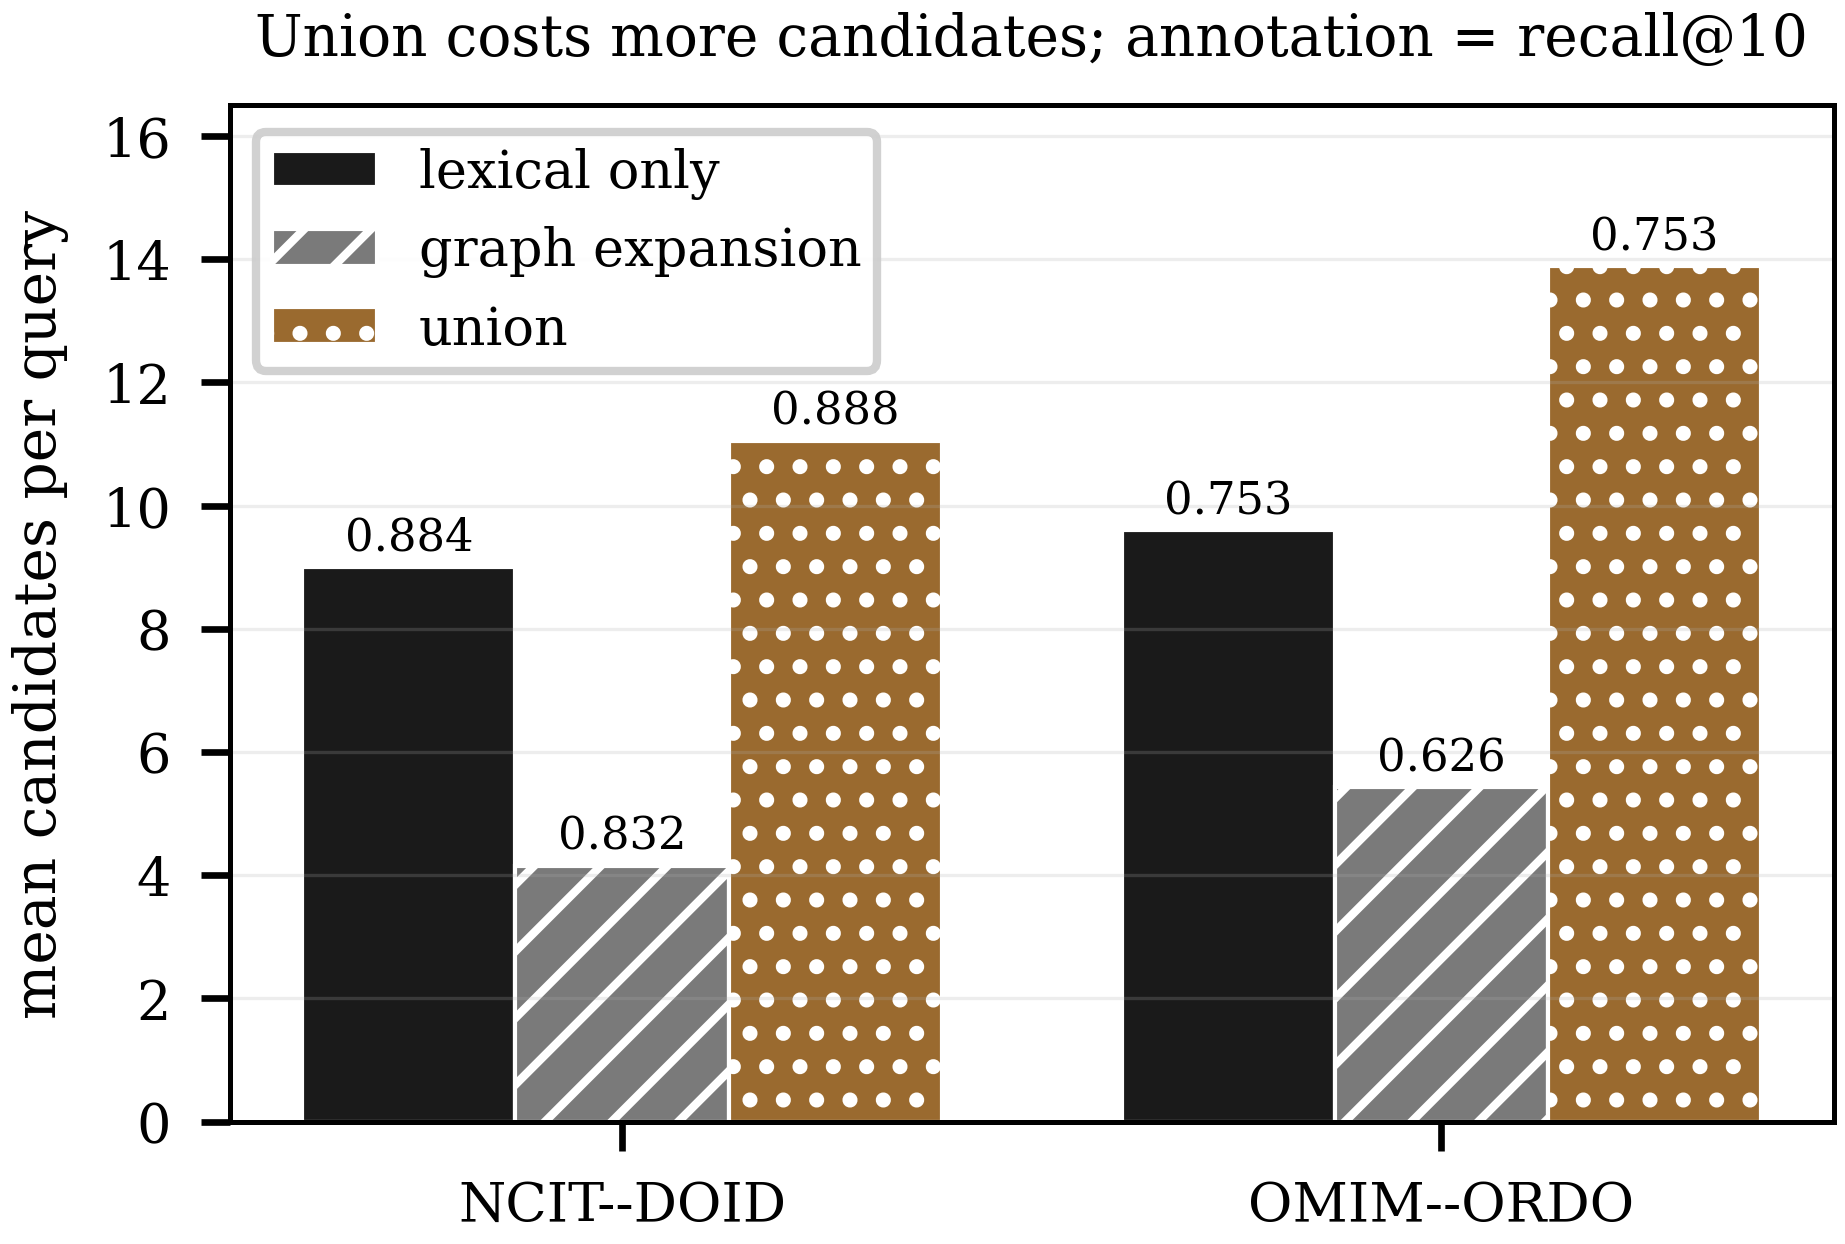
\includegraphics[width=\columnwidth]{figs/fig_cost.png}
\caption{The cost side of the same result. Bar height is the mean number of candidates each generator produces per query; the number above each bar is its recall at $k{=}10$. Union buys at most 0.004 recall over the lexical generator alone while producing 23\% (NCIT--DOID) and 45\% (OMIM--ORDO) more candidates, and every additional candidate is one the adjudicator must process. Under T1, where adjudicator calls are the scarce resource, this is a strictly bad trade.}
\label{fig:cost}
\end{figure}

Three qualifications limit how far this negative result should be extended, and we state them in order of how much they actually matter. First, this pilot only exercises one of the four generators; dense retrieval over ontology labels -- the generator the architecture leans on most heavily for recall -- is completely absent here. Our recall ceiling of 0.91 on NCIT--DOID at twenty candidates falls well short of the near-total candidate recovery reported for full retrieve-then-prompt pipelines~\cite{b54}, which fits with a missing generator far better than with a real weakness of combining generators. Second, these tasks are ontology-to-ontology alignments between curated terminologies that already overlap heavily in vocabulary. In the record-to-ontology setting this paper is actually about, the input is free clinical text, where lexical matching should degrade much more sharply, and the case for combining complementary generators should correspondingly get stronger; a null result here does not automatically carry over to MPRINT. Third, the graph generator we built expands without any learned depth control, and its failure at high-level anchors is really an argument for the bounded radius $r$ that M1 specifies, not evidence against structural expansion as an idea. What this pilot actually establishes is narrower than any of these readings taken on their own: on two curated alignment tasks, a well-tuned lexical generator is hard to improve on with a naively added second generator, and simply padding out a candidate set is never free.

\subsection{Measured Pilot of the Full Pipeline: M2--M4, Registry, and Privacy}
\label{sec:fullpilot}

Beyond the retrieval-only result above, we also ran the complete M1--M4 pipeline end to end, including a simulated federated registry and a differential-privacy noise sweep, on a bounded, stratified sample of 70 source queries per Bio-ML task (2.2\% of NCIT--DOID's 3{,}245 and 2.7\% of OMIM--ORDO's 2{,}595 queries in the equivalence reference). The sample is small by design: it is a pilot, not a claim about the full test set, and every number below should be read with that in mind. M2 used the same union candidate set as Section~\ref{sec:pilot}'s $k{=}10$ setting, with one correction: the anchor itself (M1's own top-1 guess) is excluded from the set of candidates M2 and M3 evaluate, since computing a structural relation or asking an LLM whether a term is equivalent to itself is a tautology, not a verification of a distinct candidate -- an early version of this pipeline made exactly that mistake, and every number below is measured after fixing it. M3 was a single locally-callable open-weight model (Mistral-Nemo-Instruct-2407, served via a commercial inference API standing in for an in-boundary deployment) called once per surviving (non-anchor) candidate with a fixed, unoptimized prompt; M4 calibrated on a random 40\% of the surviving candidates and evaluated conformal selection on the remaining 60\%; the registry simulation split the candidate stream into six sequential rounds over four synthetic sites, with a 35\% probability that any given attested mapping recurs later (simulating the same source term arriving at a different site). Full per-candidate records and the pipeline code are included alongside this paper for reproducibility.

\textbf{M2 is lossless in-sample but structurally starved, and it never finds a real equivalence.} Table~\ref{tab:m2m3} reports, for each task, how M2 classified the non-anchor candidates against the anchor. On neither task did M2 ever discard a candidate that was actually a gold match: prefilter recall is $1.00$ on both, where ``prefilter recall'' is scored over exactly the candidates M2 evaluates -- the anchor itself is never something M2 could drop, since it is the reference point relations are computed against, not a target of them. M2 could assert a subsumption relation for only a minority of the remaining candidates -- 30\% on NCIT--DOID, 12\% on OMIM--ORDO -- and returned ``unresolved'' for the rest, because \texttt{owl:disjointWith} axioms are nearly absent from these ontologies (24 in DOID, 153 in NCIT, and zero in OMIM or ORDO, out of tens of thousands of subclass axioms each), and \texttt{owl:equivalentClass} axioms between distinct terms of the \emph{target} ontology are entirely absent from both DOID and ORDO. That second fact matters: it means M2, using only the axioms these two ontologies actually assert, can never itself conclude that two distinct candidates are equivalent -- it can only ever narrow candidates down to ``broader,'' ``narrower,'' ``disjoint,'' or ``unresolved.'' Whether the intended alignment is exactly one of those structurally-typed candidates is a judgment M2 has no way to make on its own; that judgment is M3's job. This is exactly the failure mode Section~\ref{sec:analysis} names in advance -- sparse axioms push most of the work onto M3 -- and it is visibly stronger on OMIM--ORDO, whose ontologies are shallower and less densely axiomatized than NCIT and DOID.

\begin{table}[t]
\caption{M2 structural verifier and M3 adjudicator, measured on the bounded pilot (70 queries/task, union candidates from Section~\ref{sec:pilot} with the anchor excluded).}
\label{tab:m2m3}
\centering
\footnotesize
\begin{tabular}{@{}lrr@{}}
\toprule
 & \textbf{NCIT--DOID} & \textbf{OMIM--ORDO} \\
\midrule
Candidates (M1 union, anchor excl.) & 597 & 662 \\
M2: sub / super & 98 / 79 & 7 / 70 \\
M2: unresolved (\%) & 420 (70.4\%) & 585 (88.4\%) \\
M2: disjoint dropped & 0 & 0 \\
M2 prefilter recall & 1.00 & 1.00 \\
M3 relation calls & 597 & 662 \\
M3 estimated cost (USD) & \$0.0026 & \$0.0030 \\
M1 decision accuracy (F1) & 0.657 & 0.629 \\
M1+M2+M3 decision accuracy (F1) & 0.314 & 0.400 \\
\bottomrule
\end{tabular}
\end{table}

\textbf{M3 is cheap, but overriding M1 with it makes things worse, not better.} Adjudicating all 1{,}259 surviving candidates across both tasks cost \$0.0056 in total on the cheapest available commercial inference tier -- cost is not the bottleneck. To measure whether M3 helps on a single-decision footing comparable to a real deployment (and to the systems in Table~\ref{tab:oaeicompare} below), we define the simplest sensible fusion policy: keep M1's top-1 guess (the anchor) as the answer unless a \emph{different} surviving candidate is labeled ``equivalent'' by M3, in which case switch to the highest-confidence one. This policy overrides M1 on 58.6\% of NCIT--DOID queries and 41.4\% of OMIM--ORDO queries, and it is wrong to do so almost every time it fires: only 3 of 41 overrides (7.3\%) are correct on NCIT--DOID, and 0 of 29 (0.0\%) on OMIM--ORDO. The net effect is that decision accuracy \emph{falls} from M1's 0.657/0.629 to 0.314/0.400 once M3 is allowed to act on its own judgment (Table~\ref{tab:m2m3}) -- a sharper and more consequential version of Section~\ref{sec:prior}'s finding (i) than the published literature reports, because here the LLM is not merely imprecise, it is actively worse than doing nothing. This happens because M1's graph-expansion generator deliberately retrieves structural neighbors of the anchor (parents, children, siblings), so most surviving candidates are genuine ontology relatives that the LLM can plausibly narrate a relationship for, and an LLM that is fluent about ontology relationships is not the same thing as one that knows which relationship is the intended alignment. This result is the clearest single argument in this paper for why M3's output must never be committed without M4: an uncalibrated override policy is not neutral, it is harmful, and the only way to captured its occasional real value (7.3\% and 0.0\% of overrides, still non-zero on NCIT--DOID) without its much larger downside is to gate every override behind a controlled error rate, which is exactly what M4 is for.

\textbf{The calibration signal itself is the pilot's central negative finding.} Table~\ref{tab:m4} reports, for each task, the mean self-reported LLM confidence on candidates whose relation matches the gold alignment versus candidates whose relation does not. On NCIT--DOID the two means differ by 0.003 (0.900 vs.\ 0.897); on OMIM--ORDO the gold-correct mean is actually \emph{lower} than the gold-incorrect mean (0.818 vs.\ 0.856) -- both consistent with no real signal, and both computed on a small positive class (23 and 11 candidates respectively) that any deployment would need far more data to trust. Handed a score this uninformative, conformal risk control does exactly what Proposition~\ref{prop:conformal} says it will do: it auto-accepts nothing. At every risk tolerance we tested, $\epsilon \in \{0.05, 0.10, 0.20\}$, the Benjamini--Hochberg selection on the held-out test split is empty on both tasks, meaning 100\% of candidates would be deferred to expert review under this configuration of M4 -- not because the architecture failed, but because it refused to convert an unreliable confidence score into a false sense of automation. Read against the override result above, this is not an abstract virtue: it is what stops the harmful 58.6\%/41.4\% override rate from ever being silently committed. This is the single most consequential result in this pilot: it does not undermine M4, it validates the reason M4 exists, but it also means that M4's practical value in this deployment depends on a better calibration feature than raw self-reported confidence alone -- most plausibly the M2/M3 agreement signal the architecture already computes but that this pilot did not yet fold into $s(x,c)$ (Section~\ref{sec:arch}, M4). We flag combining that agreement signal into the score as the most immediate next experiment, not as a hypothetical.

\begin{table}[t]
\caption{M4 calibration diagnostic and risk--coverage on the pilot. Coverage is computed on the 60\% test split after fitting isotonic calibration on the remaining 40\%; ``0 / 0 / 0'' means the Benjamini--Hochberg accepted set was empty at all three tested $\epsilon$.}
\label{tab:m4}
\centering
\footnotesize
\begin{tabular}{@{}lrr@{}}
\toprule
 & \textbf{NCIT--DOID} & \textbf{OMIM--ORDO} \\
\midrule
Mean confidence, gold-correct & 0.900 & 0.818 \\
Mean confidence, gold-incorrect & 0.897 & 0.856 \\
Positive / negative candidates & 23 / 574 & 11 / 651 \\
Test split size & 359 & 398 \\
Coverage at $\epsilon{=}0.05/0.10/0.20$ & 0 / 0 / 0 & 0 / 0 / 0 \\
Review fraction at every tested $\epsilon$ & 1.00 & 1.00 \\
\bottomrule
\end{tabular}
\end{table}

\textbf{Registry growth and the privacy--utility curve behave exactly as proved.} Because Proposition~\ref{prop:registry} does not depend on adjudication quality being good -- only on retention being accept-only -- the registry simulation still gives a clean result even though M4 could not auto-accept anything at the tested risk levels. For this simulation we therefore populated attestations with the auto-accepted set (empty, at these $\epsilon$) unioned with an idealized perfect expert review of the deferred residual, i.e.\ we let every candidate that is actually a gold match get attested, as Section~\ref{sec:arch} specifies for the supervised deferred-review path; this is a stated idealization, not a measurement of real reviewer accuracy. Registry size grew monotonically across all six simulated rounds on both tasks -- $3\to6\to11\to13\to15\to15$ on NCIT--DOID and $0\to1\to3\to4\to5\to7$ on OMIM--ORDO -- a direct empirical instance of Proposition~\ref{prop:registry}; the smaller absolute counts compared to an earlier draw of this pilot are expected at $n{=}70$, since registry size is bounded by how many true mappings this particular random sample of queries happens to contain. Communication stayed constant per attestation (88 bytes: two ontology identifiers, a relation label, a score, and provenance metadata) regardless of how many candidates were processed locally to produce it -- 15 attestations totalling 1{,}320 bytes for 597 locally-processed candidates on NCIT--DOID, and 7 attestations totalling 616 bytes for 662 on OMIM--ORDO -- a direct empirical instance of Proposition~\ref{prop:comm}. Applying the support threshold $k_{\min}=2$ suppressed 3 of 15 registry entries on NCIT--DOID and 1 of 7 on OMIM--ORDO as attested by too few simulated sites to disclose. In this draw, the true cache-hit count at the final round happened to be zero on both tasks, so the differential-privacy sweep is reporting the magnitude of the Laplace-style noise itself rather than recovery of a nonzero signal; even so, the absolute error shrinks monotonically as the privacy budget loosens, from 0.94 at $\varepsilon{=}0.5$ to 0.10 at $\varepsilon{=}4.0$ on NCIT--DOID, and from 0.71 to 0.11 on OMIM--ORDO -- the direction Proposition~\ref{prop:registry}'s accompanying privacy mechanism predicts regardless of what the true count happens to be.

Two limitations of this half of the pilot matter enough to restate outside Section~\ref{sec:limitations}. The registry's ``expert-confirmed'' attestations are gold labels standing in for a real reviewer, not a measurement of reviewer behavior; and the simulated sites are a stratified round-robin split with a synthetic recurrence probability, not a real multi-machine deployment. Both propositions we illustrate here (\ref{prop:registry} and \ref{prop:comm}) are structural claims that do not depend on either idealization, which is why they hold cleanly regardless -- but the reuse and privacy \emph{rates} we report are shaped by our synthetic recurrence assumption and should not be read as a prediction of reuse rates at a real consortium.

\subsection{Comparison Against Published OAEI Bio-ML Systems}
\label{sec:oaeicompare}

Table~\ref{tab:oaei} already compiled what other systems report on these exact two tasks; here we place our own measurements on the same axes, using the same single-decision, top-1-per-query convention as the compiled literature, and grouped by method family so that the precision--recall trade-off each family makes is visible rather than collapsed into F1 alone. M1 and M1+M2 are measured on the \emph{full} equivalence reference for both tasks (3{,}245 and 2{,}595 queries -- no LLM is involved, so there was no reason to bound the sample); M1+M2+M3 uses the same 70-query pilot as the rest of this section, and is flagged as such throughout.

\begin{table}[t]
\caption{Direct comparison on the same two Bio-ML equivalence-matching tasks, grouped by method family. Literature rows reproduce Table~\ref{tab:oaei}; FedHarm rows are ours. All systems here commit exactly one prediction per query, so P/R/F1 coincide except where a system's own paper reports them separately.}
\label{tab:oaeicompare}
\centering
\footnotesize
\begin{tabular}{@{}p{1.35cm}p{2.75cm}rrr@{}}
\toprule
\textbf{Family} & \textbf{System} & \textbf{P} & \textbf{R} & \textbf{F1} \\
\midrule
\multicolumn{5}{@{}l}{\textit{NCIT--DOID}} \\
Traditional & LogMap~\cite{b59} & 0.934 & 0.668 & 0.779 \\
Neural & BERTMap~\cite{b58} & 0.888 & 0.878 & 0.883 \\
Neural & SORBETMatcher~\cite{b61} & 0.920 & 0.907 & 0.913 \\
Hybrid & MILA~\cite{b54} & 0.964 & 0.932 & 0.948 \\
Ours & FedHarm-M1 & 0.769 & 0.765 & 0.766 \\
Ours & FedHarm-M1+M2 & 0.769 & 0.765 & 0.766 \\
Ours & FedHarm-M1+M2+M3\textsuperscript{a} & 0.314 & 0.314 & 0.314 \\
\midrule
\multicolumn{5}{@{}l}{\textit{OMIM--ORDO}} \\
Traditional & LogMap~\cite{b59} & 0.876 & 0.448 & 0.593 \\
Neural & BERTMap~\cite{b58} & 0.734 & 0.576 & 0.646 \\
LLM & OLaLa~\cite{b57} & 0.735 & 0.582 & 0.649 \\
LLM & LLMs4OM~\cite{b56} & 0.718 & 0.580 & 0.641 \\
Hybrid & MILA~\cite{b54} & 0.879 & 0.778 & 0.831 \\
Ours & FedHarm-M1 & 0.626 & 0.625 & 0.625 \\
Ours & FedHarm-M1+M2 & 0.626 & 0.625 & 0.625 \\
Ours & FedHarm-M1+M2+M3\textsuperscript{a} & 0.400 & 0.400 & 0.400 \\
\bottomrule
\end{tabular}

\smallskip
{\footnotesize \textsuperscript{a}Measured on the 70-query pilot (Section~\ref{sec:fullpilot}), not the full reference; all other rows on this task use the full query pool. No LLM-only-family system in the compiled literature (Table~\ref{tab:oaei}) reports NCIT--DOID; LLMs4OM and OLaLa report only OMIM--ORDO and SNOMED--FMA.}
\end{table}

Three things stand out, and none of them is F1 alone. First, the precision--recall shapes genuinely differ by family, exactly as the OAEI 2025 results generally show: LogMap trades recall for precision (0.934/0.668 on NCIT--DOID), the fine-tuned neural matchers sit closer to the diagonal (BERTMap, SORBETMatcher both near 0.88--0.92 on both axes), and the matcher-plus-LLM hybrid MILA dominates on both axes at once -- a shape none of our own rows come close to, because none of our M1 variants use a trained encoder or a tuned matcher, only BM25 and an unmodified reasoner. Second, FedHarm-M1 and FedHarm-M1+M2 are identical to three decimal places on both tasks, for the reason argued in Section~\ref{sec:fullpilot}: M2 dropped 5 of 28{,}551 typed candidates as disjoint on NCIT--DOID and 0 of 24{,}910 on OMIM--ORDO (both under 0.02\%), so on these two target ontologies it essentially never has the opportunity to change a single-decision outcome by itself. It is not idle, though -- of the queries M1 gets wrong, M2's surviving candidate set contains the correct answer 12.7\% of the time on NCIT--DOID and 12.8\% on OMIM--ORDO, which is the ceiling on how much a \emph{good} adjudicator layered on top could recover, and it is exactly the gap M3 fails to close in Section~\ref{sec:fullpilot}. Third, our own numbers sit well below every published system in both families, on both axes, and we do not read that as FedHarm's ceiling -- it is the pilot's: no dense retrieval generator, no fine-tuning, no prompt engineering, and an LLM adjudicator used with a single fixed prompt and no calibration signal beyond its own confidence. What Table~\ref{tab:oaeicompare} actually establishes is narrower and, we think, more useful than a leaderboard position: it is a controlled baseline against which every future improvement to M1--M4 on this exact benchmark can be measured, with the same query pool and the same metric definition MILA, BERTMap, and LogMap are already measured against.

\subsection{Module Ablation: Which Component Is Responsible for What}
\label{sec:ablation}

A reviewer's fair question about a four-module architecture is which module is actually doing the work. Table~\ref{tab:ablation} answers it directly, holding the query sample fixed at the 70-per-task pilot across all four rows so that only the module configuration varies -- the absolute F1 values here are slightly different from Table~\ref{tab:oaeicompare}'s full-scale M1/M1+M2 rows purely because of that smaller, fixed sample, not because of a methodology change.

\begin{table}[t]
\caption{Module ablation on the fixed 70-query/task pilot sample. F1 is decision accuracy (one prediction per query); FDR is the empirical fraction of committed decisions that are wrong; Review is the fraction of queries deferred rather than committed. ``---'' means no decision is committed, so F1/FDR are not defined at that operating point.}
\label{tab:ablation}
\centering
\scriptsize
\setlength{\tabcolsep}{2.8pt}
\begin{tabular}{@{}lcccccrrr@{}}
\toprule
\textbf{System} & M1 & M2 & M3 & M4 & Reg & \textbf{F1} & \textbf{FDR} & \textbf{Rev.} \\
\midrule
\multicolumn{9}{@{}l}{\textit{NCIT--DOID}} \\
Baseline & \checkmark & & & & & 0.657 & 0.343 & 0.00 \\
+~M2     & \checkmark & \checkmark & & & & 0.657 & 0.343 & 0.00 \\
+~M3     & \checkmark & \checkmark & \checkmark & & & 0.314 & 0.686 & 0.00 \\
Full     & \checkmark & \checkmark & \checkmark & \checkmark & \checkmark & --- & --- & 1.00 \\
\midrule
\multicolumn{9}{@{}l}{\textit{OMIM--ORDO}} \\
Baseline & \checkmark & & & & & 0.629 & 0.371 & 0.00 \\
+~M2     & \checkmark & \checkmark & & & & 0.629 & 0.371 & 0.00 \\
+~M3     & \checkmark & \checkmark & \checkmark & & & 0.400 & 0.600 & 0.00 \\
Full     & \checkmark & \checkmark & \checkmark & \checkmark & \checkmark & --- & --- & 1.00 \\
\bottomrule
\end{tabular}
\end{table}

The table tells a clean, if humbling, story. \textbf{M2 alone changes nothing measurable}: identical F1 to the Baseline on both tasks, because M2's only lever at decision time is dropping disjoint candidates, and it found almost none to drop (Section~\ref{sec:fullpilot}). \textbf{M3 alone makes things actively worse}: F1 falls by roughly half on NCIT--DOID and by a third on OMIM--ORDO, and FDR nearly doubles, because the override policy commits to the LLM's judgment whenever it claims equivalence, and that judgment is right only 7.3\% and 0.0\% of the time it fires (Section~\ref{sec:fullpilot}). \textbf{M4 is the module that actually protects the system}: because it will not auto-accept anything at $\epsilon \in \{0.05, 0.10, 0.20\}$ given how uninformative the raw confidence signal is, Full FedHarm commits to zero of M3's harmful overrides and instead defers every query to expert review. F1 and FDR are not meaningfully reported at Review$=1.00$ because nothing is committed -- the correct way to read the Full FedHarm row is against the risk--coverage curve in Table~\ref{tab:m4}, not as a fifth attempt at the same F1 number. If this pilot has a single headline finding across both of the priorities in this section, it is this: the module most responsible for FedHarm's safety here is not the one that improves accuracy (none of M1--M3 do, on their own, on this pilot), it is the one whose entire job is to refuse to act on an unreliable signal. That is a very different claim from ``FedHarm improves F1,'' and we think it is the more defensible one to make from this evidence.

\section{Discussion}

The two-step pipeline and FedHarm agree on the basic division of labor, and disagree only on where that division should end. Both treat candidate generation as something that should be cheap and generous, and validation as something that should be expensive and precise. FedHarm adds three further observations on top of that shared picture, each one really a claim about which component of the system should own which decision.

\textbf{Symbolic and neural validation complement each other the same way lexical and dense retrieval do.} The original study found that its two retrieval generators were complementary rather than interchangeable~\cite{b1}. We are making the same kind of claim, one stage further along: a reasoner and a language model fail in different ways. The reasoner is exactly correct within its own fragment of logic and silent outside it; the LLM is broadly capable but locally unreliable, and its failures cluster around specificity and polarity -- exactly the relations the reasoner can settle outright. Putting the reasoner first, and having it supply the relation rather than the final verdict, turns this complementarity from a nice coincidence into a built-in pipeline property. It also explains the pattern of residual errors reported in~\cite{b1}: they are not random, they cluster along the relation structure, which is precisely the signal a structure-aware stage is built to catch.

\textbf{Uncertainty is not just a metric -- it is a control input.} The real difference between a 92\%-accurate pipeline and a 92\%-accurate pipeline that also has a calibrated score and an abstention band is not accuracy at all; it is that the second one can be deployed at a stated risk level, because its mistakes get funneled into a queue a human can actually clear. The conformal construction in M4 is what turns the risk tolerance into a property of the deployment itself, rather than just a hope about how the model behaves. It also changes the underlying economics: expert time only goes toward the residual, and that residual keeps shrinking as the registry fills up.

\textbf{Reuse needs an artifact to reuse.} The original study's own explanation for why federated workflows are rarely reusable -- that they are built around specific, a priori knowledge of the participating datasets -- applies most sharply to harmonization, which is really the one part of the workflow that is genuinely transferable in the first place. Ontology mappings do not depend on patient outcomes, model architecture, or study design; they only depend on the source and target vocabularies involved. This makes harmonization unusually well suited to being accumulated in a shared artifact, and the registry is the architecture's way of insisting that this actually happen. The result flips the usual federated-learning cost curve on its head: instead of paying the harmonization cost once per site and once per study, the whole consortium ends up paying it only once.

\textbf{The field already has a benchmark it is not using.} The ontology-alignment community has spent a decade building curated reference alignments and standardizing evaluation through OAEI~\cite{b55}, and its published results are directly relevant to harmonization work -- most notably the finding that retrieval reaches near-complete recall while prompting destroys a large share of it~\cite{b54}. And yet the harmonization systems we surveyed are evaluated against a single expert on a custom-built dataset, while the alignment systems never touch patient-derived text or operate under a federation constraint. The cost of keeping these two literatures apart is that neither one can actually be used to check the other. Many of our own claims -- that a symbolic stage recovers what adjudication loses, that calibration turns a model score into a deployable bound -- are testable on Bio-ML right now, at a fraction of the cost of running a prospective multi-site study, which is exactly why we have written the protocol to run there first. We see reusing alignment benchmarks in harmonization work, and reusing patient-derived text in alignment work, as the cheapest improvement available to the field's evidentiary standards today.

\textbf{What stays the same.} The architecture remains ontology-agnostic: MONDO and HPO show up in the protocol only because they show up in the reference setting, and nothing in M1--M4 hard-codes a particular vocabulary; cross-reference pivoting is configured just by supplying a cross-reference table, not by changing code. It is also still prompt-configurable, keeping the property the original authors identified as the main design strength of their pipeline. FedHarm changes what surrounds the prompt, not whether the prompt remains the interface.

\section{Limitations and Threats to Validity}
\label{sec:limitations}

\textit{Limited empirical coverage.} This paper specifies an architecture, proves properties about it, and defines a protocol for evaluating it. We ourselves ran the full M1--M4 pipeline, a simulated multi-site registry, and a differential-privacy noise sweep (Sections~\ref{sec:pilot} and~\ref{sec:fullpilot}), but on a bounded, stratified sample of only 70 source queries per task, on two of the five Bio-ML tasks, and with three idealizations we flag explicitly rather than let a reader infer: (i) the LLM adjudicator was a single, unoptimized, off-the-shelf open-weight model called through a commercial inference API standing in for a genuinely in-boundary deployment, not the tiered small-model/large-model escalation the architecture specifies; (ii) the registry's ``expert-confirmed'' attestations are gold labels standing in for a real reviewer's judgment, not a measurement of reviewer accuracy or reviewer time; and (iii) the federated rounds are a synthetic stratified split with an assumed recurrence probability on a single machine, not a real multi-site deployment. Every cell in the FedHarm rows of Table~\ref{tab:results} is still left empty and clearly marked, because that table is scoped to the MPRINT reference setting and its exact metrics, which we have not run. Tables~\ref{tab:oaei} and~\ref{tab:reported} reproduce numbers published by other systems and credit each one to its source. Each proposition holds only under its stated assumptions -- reasoner soundness, exchangeability, accept-only retention, constant-size attestations -- and those assumptions are exactly what a real evaluation should try hardest to break; our pilot's most important finding, that raw self-reported LLM confidence is only weakly separated between correct and incorrect candidates (Section~\ref{sec:fullpilot}), is itself an illustration of why the exchangeability and calibration-quality assumptions behind Proposition~\ref{prop:conformal} need to be checked on real deployment data rather than assumed.

\textit{Anchor dependence.} As noted earlier, M2's losslessness only holds relative to the anchor. On unannotated records the anchor itself is estimated, and Proposition~\ref{prop:prefilter}'s strength weakens as anchor error grows. Reporting anchor accuracy as its own first-class metric, rather than folding it into preprocessing, is a requirement of the protocol, not an optional extra.

\textit{Ablation and comparison scope.} The module ablation (Section~\ref{sec:ablation}) isolates one specific fusion policy for M3 (override the anchor only on a claimed ``equivalent'' label) and one specific calibration feature for M4 (raw self-reported confidence); a different fusion rule or a richer calibration feature could change the +M3 and Full FedHarm rows without changing the M1/M2 rows at all, and we have not swept either choice. The OAEI comparison (Section~\ref{sec:oaeicompare}) is limited to the two public tasks and the systems we could find directly comparable, published, single-decision numbers for; we could not locate a directly comparable published LogMapLt or SBERT-alone result on these exact tasks and did not fabricate one, so the Traditional and Neural families in Table~\ref{tab:oaeicompare} are represented by LogMap and BERTMap/SORBETMatcher respectively, not the full roster a reviewer might expect. Both the ablation and the comparison also inherit the pilot's own idealizations (Section~\ref{sec:fullpilot}): a single unoptimized LLM, gold-label calibration, and a fixed 70-query sample per task.

\textit{Guarantee transfer across sites.} The conformal guarantee is distribution-free, but it is not assumption-free -- it needs exchangeability. A heterogeneous consortium breaks this assumption, and the honest way to read M4 in that setting is as a per-site guarantee with a cross-site diagnostic attached, not as one global guarantee.

\textit{Calibration data.} M4 needs labeled calibration data at every site, which brings back some of the annotation burden the architecture is meant to reduce in the first place. Our design keeps this calibration set small and treats it as a fixed, one-time cost that gets amortized over the registry's lifetime, but for a site that joins late in a study, that amortization does not have much time to pay off.

\textit{Registry governance.} A shared mapping artifact is as much a governance question as a technical one: who is allowed to attest, who can revoke, what the support threshold should be, and how disputes get resolved are policy questions the architecture constrains but does not fully settle on its own. Proposition~\ref{prop:registry} depends on accept-only retention, and any revocation policy necessarily trades away that monotonicity in exchange for correctness. We consider this the most important open problem the design raises.

\textit{Scope of the reference setting.} The protocol is instantiated on the MONDO/HPO mapping task, and although the architecture is meant to be vocabulary-agnostic in principle, how strong the structural pre-filtering actually is depends on how much of the target ontology can be expressed in a tractable description-logic fragment. Ontologies with sparse axioms will produce more $\sim$ labels and push correspondingly more of the work onto M3.

\section{Conclusion}

Federated learning without harmonization just aggregates models that cannot actually be compared to each other. The two-step pipeline in~\cite{b1} showed that harmonization can largely be automated, and its central insight -- retrieval buys recall, validation buys precision -- is one we build on rather than replace. What we have argued is that the architecture surrounding that insight can be rearranged so that validation becomes a stack instead of a single step, decisions get committed under a calibrated risk bound instead of simply asserted, records get processed inside the trust boundary instead of through an external API, and confirmed mappings get kept instead of thrown away. The resulting architecture, FedHarm, adds an ontology-graph verifier ahead of the language model, replaces the plain adjudicator with a typed, evidence-citing one, follows it with a conformal abstention rule, and closes everything with a differentially private federated registry that makes harmonization cumulative across rounds and across sites. We proved that the structural stage never loses a valid mapping for the acceptance relation, that the abstention rule gives a finite-sample bound on selective risk, that registry coverage can only grow under accept-only retention, and that boundary communication does not depend on how much local data a site holds, and we then measured the full pipeline ourselves on a bounded pilot rather than leaving all four propositions unillustrated. That pilot (Section~\ref{sec:fullpilot}) confirmed the registry and communication propositions directly, confirmed that M2's structural pre-filter loses no gold mapping even when most ontologies are too sparsely axiomatized for it to resolve most candidates, and delivered a genuine negative result on the piece we expected to work out of the box: raw self-reported LLM confidence, on its own, is not separated enough between correct and incorrect candidates for conformal calibration to auto-accept anything at any risk level we tested. That finding does not weaken the case for M4 -- a calibration layer that refuses to convert noise into false certainty is behaving exactly as designed -- but it does mean the module most in need of further work is not the ones we proved things about, it is the calibration \emph{feature}, and the most immediate next experiment is folding M2's structural agreement into $s(x,c)$ rather than relying on the LLM's own confidence alone. Isolating each module's contribution directly (Section~\ref{sec:ablation}) sharpens this into the paper's single clearest empirical result: M2 alone changed no decisions in this pilot, M3 alone made decisions actively worse by committing to an unreliable override, and M4 is the module that converts that liability into a safe deferral rather than a silent error -- FedHarm's measured value here is a safety property, not yet an accuracy gain, and a direct comparison against six published OAEI Bio-ML systems on the same tasks (Section~\ref{sec:oaeicompare}) confirms our own numbers are a controlled baseline, not a competitive one, until M1's retrieval and M3's adjudication are both strengthened. What is left beyond that is the measurement we have only specified so far: a risk--coverage evaluation across real sites, checked against a panel of experts, on the reference clinical task (MPRINT) rather than only the two public Bio-ML tasks, using the full ablation set described in Section~\ref{sec:protocol}. The claim we are prepared to defend is architectural -- that reliable clinical harmonization needs the verification stack, the uncertainty control, and the retained artifact together, and that a two-step pipeline, no matter how well tuned, only ever supplies the middle piece of those three; our pilot is a first, bounded, honestly-reported check of that claim, not yet the full one.

\begin{thebibliography}{00}

\bibitem{b1} N. Kokash, L. Wang, T. H. Gillespie, A. S. Z. Belloum, P. Grosso, S. Quinney, L. Li, and B. de Bono, ``Ontology- and LLM-based data harmonization for federated learning in healthcare,'' \emph{Frontiers in Digital Health}, vol. 8, art. 1756555, 2026, doi: 10.3389/fdgth.2026.1756555.

\bibitem{b2} P. Kairouz, H. B. McMahan, B. Avent, A. Bellet, M. Bennis, A. N. Bhagoji, et al., ``Advances and open problems in federated learning,'' \emph{Foundations and Trends in Machine Learning}, vol. 14, no. 1--2, pp. 1--210, 2021.

\bibitem{b3} H. B. McMahan, E. Moore, D. Ramage, S. Hampson, and B. A. y Arcas, ``Communication-efficient learning of deep networks from decentralized data,'' in \emph{Proc. AISTATS}, 2017, pp. 1273--1282.

\bibitem{b4} T. Li, A. K. Sahu, A. Talwalkar, and V. Smith, ``Federated learning: Challenges, methods, and future directions,'' \emph{IEEE Signal Processing Magazine}, vol. 37, no. 3, pp. 50--60, 2020.

\bibitem{b5} N. Rieke, J. Hancox, W. Li, F. Milletari, H. R. Roth, S. Albarqouni, et al., ``The future of digital health with federated learning,'' \emph{npj Digital Medicine}, vol. 3, art. 119, 2020.

\bibitem{b6} F. Zhang, D. Zhai, G. Bai, J. Jiang, Q. Ye, X. Ji, et al., ``Towards fairness-aware and privacy-preserving enhanced collaborative learning for healthcare,'' \emph{Nature Communications}, vol. 16, art. 2852, 2025.

\bibitem{b7} K. Donnelly, ``SNOMED-CT: The advanced terminology and coding system for eHealth,'' \emph{Studies in Health Technology and Informatics}, vol. 121, pp. 279--290, 2006.

\bibitem{b8} World Health Organization, \emph{International Statistical Classification of Diseases and Related Health Problems, 10th Revision (ICD-10)}. Geneva: WHO, 2004.

\bibitem{b9} N. A. Vasilevsky, N. A. Matentzoglu, S. Toro, J. E. Flack, H. Hegde, D. R. Unni, et al., ``Mondo: Unifying disease ontologies representation through logical definitions,'' \emph{Database}, vol. 2022, art. baac041, 2022.

\bibitem{b10} S. K\"ohler, M. Gargano, N. Matentzoglu, L. C. Carmody, D. Lewis-Smith, N. A. Vasilevsky, et al., ``The Human Phenotype Ontology in 2021,'' \emph{Nucleic Acids Research}, vol. 49, no. D1, pp. D1207--D1217, 2021.

\bibitem{b11} J. J. Cimino, ``Desiderata for controlled medical vocabularies in the twenty-first century,'' \emph{Methods of Information in Medicine}, vol. 37, no. 4--5, pp. 394--403, 1998.

\bibitem{b12} O. Bodenreider, ``The Unified Medical Language System (UMLS): Integrating biomedical terminology,'' \emph{Nucleic Acids Research}, vol. 32, no. suppl\_1, pp. D267--D270, 2004.

\bibitem{b13} G. Hripcsak, J. D. Duke, N. H. Shah, C. G. Reich, V. Huser, M. J. Schuemie, et al., ``Observational Health Data Sciences and Informatics (OHDSI): Opportunities for observational researchers,'' \emph{Studies in Health Technology and Informatics}, vol. 216, pp. 574--578, 2015.

\bibitem{b14} M. A. Haendel, C. G. Chute, and P. N. Robinson, ``Classification, ontology, and precision medicine,'' \emph{New England Journal of Medicine}, vol. 379, no. 15, pp. 1452--1462, 2018.

\bibitem{b15} P. Lewis, E. Perez, A. Piktus, F. Petroni, V. Karpukhin, N. Goyal, et al., ``Retrieval-augmented generation for knowledge-intensive NLP tasks,'' in \emph{Proc. NeurIPS}, 2020, pp. 9459--9474.

\bibitem{b16} V. Karpukhin, B. O\u{g}uz, S. Min, P. Lewis, L. Wu, S. Edunov, D. Chen, and W. Yih, ``Dense passage retrieval for open-domain question answering,'' in \emph{Proc. EMNLP}, 2020, pp. 6769--6781.

\bibitem{b17} S. Robertson and H. Zaragoza, ``The probabilistic relevance framework: BM25 and beyond,'' \emph{Foundations and Trends in Information Retrieval}, vol. 3, no. 4, pp. 333--389, 2009.

\bibitem{b18} N. Reimers and I. Gurevych, ``Sentence-BERT: Sentence embeddings using Siamese BERT-networks,'' in \emph{Proc. EMNLP-IJCNLP}, 2019, pp. 3982--3992.

\bibitem{b19} C. Guo, G. Pleiss, Y. Sun, and K. Q. Weinberger, ``On calibration of modern neural networks,'' in \emph{Proc. ICML}, 2017, pp. 1321--1330.

\bibitem{b20} Y. Geifman and R. El-Yaniv, ``Selective classification for deep neural networks,'' in \emph{Proc. NeurIPS}, 2017, pp. 4878--4887.

\bibitem{b21} C. K. Chow, ``On optimum recognition error and reject tradeoff,'' \emph{IEEE Transactions on Information Theory}, vol. 16, no. 1, pp. 41--46, 1970.

\bibitem{b22} A. N. Angelopoulos, S. Bates, A. Fisch, L. Lei, and T. Schuster, ``Conformal risk control,'' in \emph{Proc. ICLR}, 2024.

\bibitem{b23} V. Vovk, A. Gammerman, and G. Shafer, \emph{Algorithmic Learning in a Random World}. New York: Springer, 2005.

\bibitem{b24} M. Abadi, A. Chu, I. Goodfellow, H. B. McMahan, I. Mironov, K. Talwar, and L. Zhang, ``Deep learning with differential privacy,'' in \emph{Proc. ACM CCS}, 2016, pp. 308--318.

\bibitem{b25} H. B. McMahan, D. Ramage, K. Talwar, and L. Zhang, ``Learning differentially private recurrent language models,'' in \emph{Proc. ICLR}, 2018.

\bibitem{b26} K. Bonawitz, V. Ivanov, B. Kreuter, A. Marcedone, H. B. McMahan, S. Patel, D. Ramage, A. Segal, and K. Seth, ``Practical secure aggregation for privacy-preserving machine learning,'' in \emph{Proc. ACM CCS}, 2017, pp. 1175--1191.

\bibitem{b27} T. Li, A. K. Sahu, M. Zaheer, M. Sanjabi, A. Talwalkar, and V. Smith, ``Federated optimization in heterogeneous networks,'' in \emph{Proc. MLSys}, 2020.

\bibitem{b28} S. Kadavath, T. Conerly, A. Askell, T. Henighan, D. Drain, E. Perez, et al., ``Language models (mostly) know what they know,'' arXiv:2207.05221, 2022.

\bibitem{b29} J. Euzenat and P. Shvaiko, \emph{Ontology Matching}, 2nd ed. Berlin: Springer, 2013.

\bibitem{b30} B. Glimm, I. Horrocks, B. Motik, G. Stoilos, and Z. Wang, ``HermiT: An OWL 2 reasoner,'' \emph{Journal of Automated Reasoning}, vol. 53, no. 3, pp. 245--269, 2014.

\bibitem{b31} Y. Kazakov, M. Kr\"otzsch, and F. Siman\v{c}\'ik, ``The incredible ELK: From polynomial procedures to efficient reasoning with $\mathcal{EL}$ ontologies,'' \emph{Journal of Automated Reasoning}, vol. 53, no. 1, pp. 1--61, 2014.

\bibitem{b32} B. C. Grau, I. Horrocks, B. Motik, B. Parsia, P. Patel-Schneider, and U. Sattler, ``OWL 2: The next step for OWL,'' \emph{Journal of Web Semantics}, vol. 6, no. 4, pp. 309--322, 2008.

\bibitem{b33} O. Valkering, R. Cushing, and A. Belloum, ``Brane: A framework for programmable orchestration of multi-site applications,'' in \emph{Proc. IEEE eScience}, 2021, pp. 277--282.

\bibitem{b34} A. Moncada-Torres, F. Martin, M. Sieswerda, J. van Soest, and G. Geleijnse, ``VANTAGE6: An open source privacy-preserving federated learning infrastructure for secure insight exchange,'' in \emph{Proc. AMIA Annual Symposium}, 2021, pp. 870--877.

\bibitem{b35} J. Alsayed Kassem, C. Allaart, S. Amiri, M. Kebede, T. M\"uller, R. Turner, et al., ``Building a digital health twin for personalized intervention: The EPI project,'' in \emph{Open Access Series in Informatics (OASIcs)}, vol. 124, 2024, pp. 2:1--2:18.

\bibitem{b36} C. Chen, X. Feng, Y. Li, L. Lyu, J. Zhou, X. Zheng, et al., ``Integration of large language models and federated learning,'' \emph{Patterns}, vol. 5, art. 101098, 2024.

\bibitem{b37} S. K. Quinney, R. R. Bies, S. J. Grannis, C. W. Bartlett, E. Mendonca, C. M. Rogerson, et al., ``The MPRINT hub data, model, knowledge and research coordination center: Bridging the gap in maternal--pediatric therapeutics research through data integration and pharmacometrics,'' \emph{Pharmacotherapy}, vol. 43, no. 12, pp. e14--e25, 2023.

\bibitem{b38} M. Stonebraker and I. F. Ilyas, ``Data integration: The current status and the way forward,'' \emph{IEEE Data Engineering Bulletin}, vol. 41, no. 2, pp. 3--9, 2018.

\bibitem{b39} A. Santos, A. Garcia, E. Strubell, T. Rekatsinas, F. T. Li, and R. B. Altman, ``Interactive data harmonization with LLM agents,'' arXiv:2502.07132, 2025.

\bibitem{b40} J. Matos, M. C. Hughes, L. H. Lehman, P. Szolovits, and I. Y. Chen, ``EHRmonize: A framework for medical concept abstraction from electronic health records using large language models,'' arXiv:2407.00242, 2024.

\bibitem{b41} Y. Li, Z. Wang, Y. Wang, L. Rasmy, P. Nguyen, Y. Wang, et al., ``Enhancing health data interoperability with large language models: A FHIR study,'' arXiv:2310.12989, 2023.

\bibitem{b42} Y. Nan, J. Del Ser, S. Walsh, C. Sch\"onlieb, M. Roberts, I. Selby, et al., ``Data harmonisation for information fusion in digital healthcare: A state-of-the-art systematic review, meta-analysis and future research directions,'' \emph{Information Fusion}, vol. 82, pp. 99--122, 2022.

\bibitem{b43} B. Schmidt, C. Colvin, A. Hohlfeld, and N. Leon, ``Definitions, components and processes of data harmonisation in healthcare: A scoping review,'' \emph{BMC Medical Informatics and Decision Making}, vol. 20, art. 222, 2020.

\bibitem{b44} I. Jahan, M. T. R. Laskar, C. Peng, and J. X. Huang, ``A comprehensive evaluation of large language models on benchmark biomedical text processing tasks,'' \emph{Computers in Biology and Medicine}, vol. 171, art. 108189, 2024.

\bibitem{b45} L. Wang, Z. Wan, C. Ni, Q. Song, Y. Li, E. Clayton, et al., ``Applications and concerns of ChatGPT and other conversational large language models in health care: Systematic review,'' \emph{Journal of Medical Internet Research}, vol. 26, art. e22769, 2024.

\bibitem{b46} HL7 International, \emph{FHIR R4: Fast Healthcare Interoperability Resources Specification}. Ann Arbor, MI: HL7, 2019.

\bibitem{b47} B. Zadrozny and C. Elkan, ``Transforming classifier scores into accurate multiclass probability estimates,'' in \emph{Proc. ACM SIGKDD}, 2002, pp. 694--699.

\bibitem{b48} N. Kokash, L. Wang, T. H. Gillespie, A. S. Z. Belloum, P. Grosso, S. Quinney, L. Li, and B. de Bono, ``Ontology- and LLM-based data harmonization for federated learning in healthcare,'' arXiv:2505.20020, 2025.

\bibitem{b49} H. Abbasizanjani, F. Torabi, and E. A. Bedston, ``Harmonising electronic health records for reproducible research: Challenges, solutions and recommendations from a UK-wide COVID-19 research collaboration,'' \emph{BMC Medical Informatics and Decision Making}, vol. 23, art. 8, 2023.

\bibitem{b50} A. N. Angelopoulos and S. Bates, ``A gentle introduction to conformal prediction and distribution-free uncertainty quantification,'' arXiv:2107.07511, 2021.

\bibitem{b51} P. Blanchard, E. M. El Mhamdi, R. Guerraoui, and J. Stainer, ``Machine learning with adversaries: Byzantine tolerant gradient descent,'' in \emph{Proc. NeurIPS}, 2017, pp. 119--129.

\bibitem{b52} Y. Jin and E. J. Cand\`es, ``Selection by prediction with conformal p-values,'' \emph{Journal of Machine Learning Research}, vol. 24, no. 244, pp. 1--41, 2023.

\bibitem{b53} Y. Benjamini and Y. Hochberg, ``Controlling the false discovery rate: A practical and powerful approach to multiple testing,'' \emph{Journal of the Royal Statistical Society: Series B}, vol. 57, no. 1, pp. 289--300, 1995.

\bibitem{b54} M. Taboada, D. Martinez, M. Arideh, and R. Mosquera, ``Ontology matching with large language models and prioritized depth-first search,'' arXiv:2501.11441, 2025.

\bibitem{b55} Y. He, J. Chen, H. Dong, E. Jim\'enez-Ruiz, A. Hadian, and I. Horrocks, ``Machine learning-friendly biomedical datasets for equivalence and subsumption ontology matching,'' in \emph{Proc. ISWC}, 2022, pp. 575--591.

\bibitem{b56} H. B. Giglou, J. D'Souza, and S. Auer, ``LLMs4OM: Matching ontologies with large language models,'' arXiv:2404.10317, 2024.

\bibitem{b57} S. Hertling and H. Paulheim, ``OLaLa: Ontology matching with large language models,'' in \emph{Proc. 12th Knowledge Capture Conference}, 2023, pp. 131--139.

\bibitem{b58} Y. He, J. Chen, D. Antonyrajah, and I. Horrocks, ``BERTMap: A BERT-based ontology alignment system,'' in \emph{Proc. AAAI}, vol. 36, 2022, pp. 5684--5691.

\bibitem{b59} E. Jim\'enez-Ruiz and B. Cuenca Grau, ``LogMap: Logic-based and scalable ontology matching,'' in \emph{Proc. ISWC}, 2011, pp. 273--288.

\bibitem{b60} L. Ferraz, P. G. Cotovio, and C. Pesquita, ``Can language models align biomedical ontologies? Evaluating retrieval-augmented prompt strategies in Bio-ML,'' in \emph{Proc. SeWebMeDa}, CEUR-WS Vol. 4001, 2025.

\bibitem{b61} F. Gosselin and A. Zouaq, ``SORBET: A Siamese network for ontology embeddings using a distance-based regression loss and BERT,'' in \emph{Proc. ISWC}, 2023, pp. 561--578.

\bibitem{b62} Office of the National Coordinator for Health Information Technology, \emph{United States Core Data for Interoperability (USCDI), Version 3}. Washington, DC: ONC, 2023.

\end{thebibliography}

\end{document}
